\section{Einfache Impulse}
\subsection*{Rechteckimpuls/ -funktion \texorpdfstring{$rect_T\left(t\right)$}{}}
\index{Impulse!Rechteck}
\begin{multicols}{2}
\begin{equation*}
x\left(t\right) = X_0 \cdot rect_T\left(t\right) 
\end{equation*}

\begin{itemize}
 \item T: Rechteckimpulsbreite \(> 0\)
 \item an den Sprungstellen nimmt der Impuls die Hälfte des max. Wertes an
\end{itemize}

\begin{center}
 % Graphic for TeX using PGF
% Title: /home/Befedo/Documents/eclipse.workspace/Formelsammlung/Elektrotechnik/Bilder/rect.dia
% Creator: Dia v0.97
% CreationDate: Tue Jan  3 07:53:56 2012
% For: Befedo
% \usepackage{tikz}
% The following commands are not supported in PSTricks at present
% We define them conditionally, so when they are implemented,
% this pgf file will use them.
\ifx\du\undefined
  \newlength{\du}
\fi
\setlength{\du}{15\unitlength}
\begin{tikzpicture}
\pgftransformxscale{0.567523}
\pgftransformyscale{-0.567523}
\definecolor{dialinecolor}{rgb}{0.000000, 0.000000, 0.000000}
\pgfsetstrokecolor{dialinecolor}
\definecolor{dialinecolor}{rgb}{1.000000, 1.000000, 1.000000}
\pgfsetfillcolor{dialinecolor}
\pgfsetlinewidth{0.100000\du}
\pgfsetdash{}{0pt}
\pgfsetdash{}{0pt}
\pgfsetbuttcap
{
\definecolor{dialinecolor}{rgb}{0.000000, 0.000000, 0.000000}
\pgfsetfillcolor{dialinecolor}
% was here!!!
\pgfsetarrowsend{stealth}
\definecolor{dialinecolor}{rgb}{0.000000, 0.000000, 0.000000}
\pgfsetstrokecolor{dialinecolor}
\draw (0.000000\du,10.000000\du)--(16.000000\du,10.000000\du);
}
\pgfsetlinewidth{0.100000\du}
\pgfsetdash{}{0pt}
\pgfsetdash{}{0pt}
\pgfsetbuttcap
{
\definecolor{dialinecolor}{rgb}{0.000000, 0.000000, 0.000000}
\pgfsetfillcolor{dialinecolor}
% was here!!!
\pgfsetarrowsend{stealth}
\definecolor{dialinecolor}{rgb}{0.000000, 0.000000, 0.000000}
\pgfsetstrokecolor{dialinecolor}
\draw (8.000000\du,10.000000\du)--(8.000000\du,1.000000\du);
}
\pgfsetlinewidth{0.100000\du}
\pgfsetdash{}{0pt}
\pgfsetdash{}{0pt}
\pgfsetmiterjoin
\pgfsetbuttcap
{
\definecolor{dialinecolor}{rgb}{1.000000, 0.000000, 0.000000}
\pgfsetfillcolor{dialinecolor}
% was here!!!
{\pgfsetcornersarced{\pgfpoint{0.000000\du}{0.000000\du}}\definecolor{dialinecolor}{rgb}{1.000000, 0.000000, 0.000000}
\pgfsetstrokecolor{dialinecolor}
\draw (0.000000\du,10.000000\du)--(5.000000\du,10.000000\du)--(5.000000\du,5.000000\du)--(11.000000\du,5.000000\du)--(11.000000\du,10.000000\du)--(15.000000\du,10.000000\du);
}}
\pgfsetlinewidth{0.100000\du}
\pgfsetdash{}{0pt}
\pgfsetdash{}{0pt}
\pgfsetbuttcap
{
\definecolor{dialinecolor}{rgb}{0.000000, 0.000000, 0.000000}
\pgfsetfillcolor{dialinecolor}
% was here!!!
\definecolor{dialinecolor}{rgb}{0.000000, 0.000000, 0.000000}
\pgfsetstrokecolor{dialinecolor}
\draw (7.500000\du,5.500000\du)--(8.500000\du,4.500000\du);
}
\pgfsetlinewidth{0.100000\du}
\pgfsetdash{}{0pt}
\pgfsetdash{}{0pt}
\pgfsetbuttcap
{
\definecolor{dialinecolor}{rgb}{0.000000, 0.000000, 0.000000}
\pgfsetfillcolor{dialinecolor}
% was here!!!
\definecolor{dialinecolor}{rgb}{0.000000, 0.000000, 0.000000}
\pgfsetstrokecolor{dialinecolor}
\draw (5.000000\du,9.500000\du)--(5.000000\du,10.500000\du);
}
\pgfsetlinewidth{0.100000\du}
\pgfsetdash{}{0pt}
\pgfsetdash{}{0pt}
\pgfsetbuttcap
{
\definecolor{dialinecolor}{rgb}{0.000000, 0.000000, 0.000000}
\pgfsetfillcolor{dialinecolor}
% was here!!!
\definecolor{dialinecolor}{rgb}{0.000000, 0.000000, 0.000000}
\pgfsetstrokecolor{dialinecolor}
\draw (11.000000\du,9.500000\du)--(11.000000\du,10.500000\du);
}
% setfont left to latex
\definecolor{dialinecolor}{rgb}{0.000000, 0.000000, 0.000000}
\pgfsetstrokecolor{dialinecolor}
\node[anchor=east] at (5.500000\du,11.000000\du){-T/2};
% setfont left to latex
\definecolor{dialinecolor}{rgb}{0.000000, 0.000000, 0.000000}
\pgfsetstrokecolor{dialinecolor}
\node[anchor=west] at (10.500000\du,11.000000\du){T/2};
% setfont left to latex
\definecolor{dialinecolor}{rgb}{0.000000, 0.000000, 0.000000}
\pgfsetstrokecolor{dialinecolor}
\node[anchor=west] at (8.500000\du,4.500000\du){};
% setfont left to latex
\definecolor{dialinecolor}{rgb}{0.000000, 0.000000, 0.000000}
\pgfsetstrokecolor{dialinecolor}
\node[anchor=west] at (8.500000\du,4.500000\du){X0};
\end{tikzpicture}

\end{center}

\end{multicols}

\subsection*{Dreiecksimpuls/ -funktion \texorpdfstring{$\Lambda_T\left(t\right)$}{}}
\index{Impulse!Dreieck}
\begin{multicols}{2}
 \begin{align*}
x\left(t\right) &= X_0 \cdot \Lambda_T\left(t\right) \\
\Lambda_T\left(t\right) &=\begin{cases}
1-\left|t/T\right| \text{ für } \left|t\right| < T\\
0 \text{ für } \left|t\right| > T
\end{cases}
\end{align*}

\begin{itemize}
 \item T: Dauer einer ansteigenden / abfallenden Flanke
\end{itemize}

\begin{center}
 % Graphic for TeX using PGF
% Title: /home/Befedo/Documents/eclipse.workspace/Formelsammlung/Elektrotechnik/Bilder/lambda.dia
% Creator: Dia v0.97
% CreationDate: Tue Jan  3 08:05:58 2012
% For: Befedo
% \usepackage{tikz}
% The following commands are not supported in PSTricks at present
% We define them conditionally, so when they are implemented,
% this pgf file will use them.
\ifx\du\undefined
  \newlength{\du}
\fi
\setlength{\du}{15\unitlength}
\begin{tikzpicture}
\pgftransformxscale{0.567523}
\pgftransformyscale{-0.567523}
\definecolor{dialinecolor}{rgb}{0.000000, 0.000000, 0.000000}
\pgfsetstrokecolor{dialinecolor}
\definecolor{dialinecolor}{rgb}{1.000000, 1.000000, 1.000000}
\pgfsetfillcolor{dialinecolor}
\pgfsetlinewidth{0.100000\du}
\pgfsetdash{}{0pt}
\pgfsetdash{}{0pt}
\pgfsetbuttcap
{
\definecolor{dialinecolor}{rgb}{0.000000, 0.000000, 0.000000}
\pgfsetfillcolor{dialinecolor}
% was here!!!
\pgfsetarrowsend{stealth}
\definecolor{dialinecolor}{rgb}{0.000000, 0.000000, 0.000000}
\pgfsetstrokecolor{dialinecolor}
\draw (8.000000\du,10.000000\du)--(8.000000\du,1.000000\du);
}
\pgfsetlinewidth{0.100000\du}
\pgfsetdash{}{0pt}
\pgfsetdash{}{0pt}
\pgfsetmiterjoin
\pgfsetbuttcap
{
\definecolor{dialinecolor}{rgb}{1.000000, 0.000000, 0.000000}
\pgfsetfillcolor{dialinecolor}
% was here!!!
{\pgfsetcornersarced{\pgfpoint{0.000000\du}{0.000000\du}}\definecolor{dialinecolor}{rgb}{1.000000, 0.000000, 0.000000}
\pgfsetstrokecolor{dialinecolor}
\draw (0.000000\du,10.000000\du)--(5.000000\du,10.000000\du)--(8.000000\du,5.000000\du)--(11.000000\du,10.000000\du)--(15.000000\du,10.000000\du);
}}
% setfont left to latex
\definecolor{dialinecolor}{rgb}{0.000000, 0.000000, 0.000000}
\pgfsetstrokecolor{dialinecolor}
\node[anchor=west] at (8.500000\du,4.500000\du){};
\pgfsetlinewidth{0.100000\du}
\pgfsetdash{}{0pt}
\pgfsetdash{}{0pt}
\pgfsetbuttcap
{
\definecolor{dialinecolor}{rgb}{0.000000, 0.000000, 0.000000}
\pgfsetfillcolor{dialinecolor}
% was here!!!
\definecolor{dialinecolor}{rgb}{0.000000, 0.000000, 0.000000}
\pgfsetstrokecolor{dialinecolor}
\draw (5.000000\du,9.500000\du)--(5.000000\du,10.500000\du);
}
\pgfsetlinewidth{0.100000\du}
\pgfsetdash{}{0pt}
\pgfsetdash{}{0pt}
\pgfsetbuttcap
{
\definecolor{dialinecolor}{rgb}{0.000000, 0.000000, 0.000000}
\pgfsetfillcolor{dialinecolor}
% was here!!!
\definecolor{dialinecolor}{rgb}{0.000000, 0.000000, 0.000000}
\pgfsetstrokecolor{dialinecolor}
\draw (11.000000\du,9.500000\du)--(11.000000\du,10.500000\du);
}
\pgfsetlinewidth{0.100000\du}
\pgfsetdash{}{0pt}
\pgfsetdash{}{0pt}
\pgfsetbuttcap
{
\definecolor{dialinecolor}{rgb}{0.000000, 0.000000, 0.000000}
\pgfsetfillcolor{dialinecolor}
% was here!!!
\pgfsetarrowsend{stealth}
\definecolor{dialinecolor}{rgb}{0.000000, 0.000000, 0.000000}
\pgfsetstrokecolor{dialinecolor}
\draw (0.000000\du,10.000000\du)--(16.000000\du,10.000000\du);
}
% setfont left to latex
\definecolor{dialinecolor}{rgb}{0.000000, 0.000000, 0.000000}
\pgfsetstrokecolor{dialinecolor}
\node[anchor=east] at (5.000000\du,11.000000\du){-T};
% setfont left to latex
\definecolor{dialinecolor}{rgb}{0.000000, 0.000000, 0.000000}
\pgfsetstrokecolor{dialinecolor}
\node[anchor=west] at (11.000000\du,11.000000\du){T};
\pgfsetlinewidth{0.100000\du}
\pgfsetdash{}{0pt}
\pgfsetdash{}{0pt}
\pgfsetbuttcap
{
\definecolor{dialinecolor}{rgb}{0.000000, 0.000000, 0.000000}
\pgfsetfillcolor{dialinecolor}
% was here!!!
\definecolor{dialinecolor}{rgb}{0.000000, 0.000000, 0.000000}
\pgfsetstrokecolor{dialinecolor}
\draw (7.500000\du,5.500000\du)--(8.500000\du,4.500000\du);
}
% setfont left to latex
\definecolor{dialinecolor}{rgb}{0.000000, 0.000000, 0.000000}
\pgfsetstrokecolor{dialinecolor}
\node[anchor=west] at (8.500000\du,4.500000\du){1};
\end{tikzpicture}

\end{center}

\end{multicols}

\section{Elementare Operationen auf zeitliche Verläufe}
\subsection*{Beeinflußung der Ordinate}

\begin{multicols}{2}
 \subsubsection*{Signaloffset \texorpdfstring{$X_{OFFS}$}{}}
  \begin{equation*}
   x_{neu}\left(t\right) = x_{alt}\left(t\right) + X_{OFFS} 
  \end{equation*}
\vfill
  \begin{center}
  % Graphic for TeX using PGF
% Title: /home/Befedo/Documents/eclipse.workspace/Formelsammlung/Elektrotechnik/Bilder/uoffs.dia
% Creator: Dia v0.97
% CreationDate: Tue Jan  3 08:17:01 2012
% For: Befedo
% \usepackage{tikz}
% The following commands are not supported in PSTricks at present
% We define them conditionally, so when they are implemented,
% this pgf file will use them.
\ifx\du\undefined
  \newlength{\du}
\fi
\setlength{\du}{15\unitlength}
\begin{tikzpicture}
\pgftransformxscale{0.567523}
\pgftransformyscale{-0.567523}
\definecolor{dialinecolor}{rgb}{0.000000, 0.000000, 0.000000}
\pgfsetstrokecolor{dialinecolor}
\definecolor{dialinecolor}{rgb}{1.000000, 1.000000, 1.000000}
\pgfsetfillcolor{dialinecolor}
\pgfsetlinewidth{0.100000\du}
\pgfsetdash{}{0pt}
\pgfsetdash{}{0pt}
\pgfsetbuttcap
{
\definecolor{dialinecolor}{rgb}{0.000000, 0.000000, 0.000000}
\pgfsetfillcolor{dialinecolor}
% was here!!!
\pgfsetarrowsend{stealth}
\definecolor{dialinecolor}{rgb}{0.000000, 0.000000, 0.000000}
\pgfsetstrokecolor{dialinecolor}
\draw (0.000000\du,10.000000\du)--(16.000000\du,10.000000\du);
}
\pgfsetlinewidth{0.100000\du}
\pgfsetdash{}{0pt}
\pgfsetdash{}{0pt}
\pgfsetbuttcap
{
\definecolor{dialinecolor}{rgb}{0.000000, 0.000000, 0.000000}
\pgfsetfillcolor{dialinecolor}
% was here!!!
\pgfsetarrowsend{stealth}
\definecolor{dialinecolor}{rgb}{0.000000, 0.000000, 0.000000}
\pgfsetstrokecolor{dialinecolor}
\draw (8.000000\du,10.000000\du)--(8.000000\du,1.000000\du);
}
\pgfsetlinewidth{0.100000\du}
\pgfsetdash{}{0pt}
\pgfsetdash{}{0pt}
\pgfsetmiterjoin
\pgfsetbuttcap
{
\definecolor{dialinecolor}{rgb}{1.000000, 0.000000, 0.000000}
\pgfsetfillcolor{dialinecolor}
% was here!!!
{\pgfsetcornersarced{\pgfpoint{0.000000\du}{0.000000\du}}\definecolor{dialinecolor}{rgb}{1.000000, 0.000000, 0.000000}
\pgfsetstrokecolor{dialinecolor}
\draw (0.000000\du,7.000000\du)--(5.000000\du,7.000000\du)--(5.000000\du,3.200000\du)--(11.000000\du,3.200000\du)--(11.000000\du,7.000000\du)--(15.000000\du,7.000000\du);
}}
% setfont left to latex
\definecolor{dialinecolor}{rgb}{0.000000, 0.000000, 0.000000}
\pgfsetstrokecolor{dialinecolor}
\node[anchor=west] at (8.500000\du,4.500000\du){};
\pgfsetlinewidth{0.100000\du}
\pgfsetdash{}{0pt}
\pgfsetdash{}{0pt}
\pgfsetbuttcap
{
\definecolor{dialinecolor}{rgb}{0.000000, 0.000000, 0.000000}
\pgfsetfillcolor{dialinecolor}
% was here!!!
\pgfsetarrowsstart{stealth}
\pgfsetarrowsend{stealth}
\definecolor{dialinecolor}{rgb}{0.000000, 0.000000, 0.000000}
\pgfsetstrokecolor{dialinecolor}
\draw (5.000000\du,7.000000\du)--(5.000000\du,10.000000\du);
}
% setfont left to latex
\definecolor{dialinecolor}{rgb}{0.000000, 0.000000, 0.000000}
\pgfsetstrokecolor{dialinecolor}
\node[anchor=east] at (5.000000\du,8.500000\du){XOFFS};
\end{tikzpicture}

  \end{center}
\end{multicols}

\begin{multicols}{2}
 \subsubsection*{Skalierungsfaktor \texorpdfstring{$V \left(V \neq 0 \right) $}{}}
 \index{Skalierungsfaktor}
  \begin{equation*}
   x_{neu}\left(t\right) = V \cdot x_{alt}\left(t\right) 
  \end{equation*}
\vfill
  \begin{center}
  % Graphic for TeX using PGF
% Title: /home/Befedo/Documents/eclipse.workspace/Formelsammlung/Elektrotechnik/Bilder/skalierung.dia
% Creator: Dia v0.97
% CreationDate: Tue Jan  3 08:22:45 2012
% For: Befedo
% \usepackage{tikz}
% The following commands are not supported in PSTricks at present
% We define them conditionally, so when they are implemented,
% this pgf file will use them.
\ifx\du\undefined
  \newlength{\du}
\fi
\setlength{\du}{15\unitlength}
\begin{tikzpicture}
\pgftransformxscale{0.567523}
\pgftransformyscale{-0.567523}
\definecolor{dialinecolor}{rgb}{0.000000, 0.000000, 0.000000}
\pgfsetstrokecolor{dialinecolor}
\definecolor{dialinecolor}{rgb}{1.000000, 1.000000, 1.000000}
\pgfsetfillcolor{dialinecolor}
\pgfsetlinewidth{0.100000\du}
\pgfsetdash{}{0pt}
\pgfsetdash{}{0pt}
\pgfsetbuttcap
{
\definecolor{dialinecolor}{rgb}{0.000000, 0.000000, 0.000000}
\pgfsetfillcolor{dialinecolor}
% was here!!!
\pgfsetarrowsend{stealth}
\definecolor{dialinecolor}{rgb}{0.000000, 0.000000, 0.000000}
\pgfsetstrokecolor{dialinecolor}
\draw (0.000000\du,10.000000\du)--(16.000000\du,10.000000\du);
}
\pgfsetlinewidth{0.100000\du}
\pgfsetdash{}{0pt}
\pgfsetdash{}{0pt}
\pgfsetbuttcap
{
\definecolor{dialinecolor}{rgb}{0.000000, 0.000000, 0.000000}
\pgfsetfillcolor{dialinecolor}
% was here!!!
\pgfsetarrowsend{stealth}
\definecolor{dialinecolor}{rgb}{0.000000, 0.000000, 0.000000}
\pgfsetstrokecolor{dialinecolor}
\draw (8.000000\du,10.000000\du)--(8.000000\du,1.000000\du);
}
\pgfsetlinewidth{0.100000\du}
\pgfsetdash{}{0pt}
\pgfsetdash{}{0pt}
\pgfsetmiterjoin
\pgfsetbuttcap
{
\definecolor{dialinecolor}{rgb}{1.000000, 0.000000, 0.000000}
\pgfsetfillcolor{dialinecolor}
% was here!!!
{\pgfsetcornersarced{\pgfpoint{0.000000\du}{0.000000\du}}\definecolor{dialinecolor}{rgb}{1.000000, 0.000000, 0.000000}
\pgfsetstrokecolor{dialinecolor}
\draw (0.000000\du,10.000000\du)--(5.000000\du,10.000000\du)--(8.000000\du,7.400000\du)--(11.000000\du,10.000000\du)--(15.000000\du,10.000000\du);
}}
% setfont left to latex
\definecolor{dialinecolor}{rgb}{0.000000, 0.000000, 0.000000}
\pgfsetstrokecolor{dialinecolor}
\node[anchor=west] at (8.500000\du,4.500000\du){};
\pgfsetlinewidth{0.100000\du}
\pgfsetdash{}{0pt}
\pgfsetdash{}{0pt}
\pgfsetmiterjoin
\pgfsetbuttcap
{
\definecolor{dialinecolor}{rgb}{0.000000, 0.000000, 1.000000}
\pgfsetfillcolor{dialinecolor}
% was here!!!
{\pgfsetcornersarced{\pgfpoint{0.000000\du}{0.000000\du}}\definecolor{dialinecolor}{rgb}{0.000000, 0.000000, 1.000000}
\pgfsetstrokecolor{dialinecolor}
\draw (0.000000\du,10.000000\du)--(5.000000\du,10.000000\du)--(8.000000\du,4.000000\du)--(11.000000\du,10.000000\du)--(15.000000\du,10.000000\du);
}}
% setfont left to latex
\definecolor{dialinecolor}{rgb}{0.000000, 0.000000, 0.000000}
\pgfsetstrokecolor{dialinecolor}
\node[anchor=west] at (8.400000\du,7.600000\du){V=1};
% setfont left to latex
\definecolor{dialinecolor}{rgb}{0.000000, 0.000000, 0.000000}
\pgfsetstrokecolor{dialinecolor}
\node[anchor=west] at (8.400000\du,4.800000\du){V!=1};
\end{tikzpicture}

  \end{center}
\end{multicols}

\subsection*{Beeinflußung der Abszisse}
\begin{multicols}{2}
 \subsubsection*{zeitliche Verschiebung \texorpdfstring{$t_0$}{}}
  \begin{equation*}
   x_{neu}\left(t\right) = x_{alt}\left(t - t_0\right) \text{ mit } t_0 = const.
  \end{equation*}
  \begin{itemize}
   \item Zusammenfassung der Offsetbehafteten Zeit \(t - t_0\) zu einer neuen Zeitbasis \(\tau = t - t_0\)
   \item \(x_{neu}\left(\tau + t_0\right) = x_{alt}\left(\tau\right) \) \\
         \(t > 0\) Verschiebung nach rechts\\
	 	 \(t < 0\) Verschiebung nach links
  \end{itemize}
 \vspace*{10mm} 
  \begin{center}
  % Graphic for TeX using PGF
% Title: /home/Befedo/Documents/eclipse.workspace/Formelsammlung/Elektrotechnik/Bilder/zeitbasis.dia
% Creator: Dia v0.97
% CreationDate: Tue Jan  3 08:30:38 2012
% For: Befedo
% \usepackage{tikz}
% The following commands are not supported in PSTricks at present
% We define them conditionally, so when they are implemented,
% this pgf file will use them.
\ifx\du\undefined
  \newlength{\du}
\fi
\setlength{\du}{15\unitlength}
\begin{tikzpicture}
\pgftransformxscale{0.577827}
\pgftransformyscale{-0.577827}
\definecolor{dialinecolor}{rgb}{0.000000, 0.000000, 0.000000}
\pgfsetstrokecolor{dialinecolor}
\definecolor{dialinecolor}{rgb}{1.000000, 1.000000, 1.000000}
\pgfsetfillcolor{dialinecolor}
\pgfsetlinewidth{0.100000\du}
\pgfsetdash{}{0pt}
\pgfsetdash{}{0pt}
\pgfsetmiterjoin
\pgfsetbuttcap
{
\definecolor{dialinecolor}{rgb}{0.000000, 0.000000, 1.000000}
\pgfsetfillcolor{dialinecolor}
% was here!!!
{\pgfsetcornersarced{\pgfpoint{0.000000\du}{0.000000\du}}\definecolor{dialinecolor}{rgb}{0.000000, 0.000000, 1.000000}
\pgfsetstrokecolor{dialinecolor}
\draw (15.000000\du,10.000000\du)--(12.029600\du,5.047900\du)--(9.000000\du,10.000000\du);
}}
% setfont left to latex
\definecolor{dialinecolor}{rgb}{0.000000, 0.000000, 0.000000}
\pgfsetstrokecolor{dialinecolor}
\node[anchor=west] at (8.500000\du,4.500000\du){};
\pgfsetlinewidth{0.100000\du}
\pgfsetdash{}{0pt}
\pgfsetdash{}{0pt}
\pgfsetmiterjoin
\pgfsetbuttcap
{
\definecolor{dialinecolor}{rgb}{1.000000, 0.000000, 0.000000}
\pgfsetfillcolor{dialinecolor}
% was here!!!
{\pgfsetcornersarced{\pgfpoint{0.000000\du}{0.000000\du}}\definecolor{dialinecolor}{rgb}{1.000000, 0.000000, 0.000000}
\pgfsetstrokecolor{dialinecolor}
\draw (0.000000\du,10.000000\du)--(3.000000\du,5.000000\du)--(6.200000\du,10.000000\du);
}}
% setfont left to latex
\definecolor{dialinecolor}{rgb}{0.000000, 0.000000, 0.000000}
\pgfsetstrokecolor{dialinecolor}
\node[anchor=west] at (0.800000\du,9.200000\du){x(t)};
% setfont left to latex
\definecolor{dialinecolor}{rgb}{0.000000, 0.000000, 0.000000}
\pgfsetstrokecolor{dialinecolor}
\node[anchor=west] at (9.800000\du,9.200000\du){x(t-T)};
\pgfsetlinewidth{0.010000\du}
\pgfsetdash{}{0pt}
\pgfsetdash{}{0pt}
\pgfsetbuttcap
{
\definecolor{dialinecolor}{rgb}{0.000000, 0.000000, 0.000000}
\pgfsetfillcolor{dialinecolor}
% was here!!!
\pgfsetarrowsstart{to}
\pgfsetarrowsend{to}
\definecolor{dialinecolor}{rgb}{0.000000, 0.000000, 0.000000}
\pgfsetstrokecolor{dialinecolor}
\draw (3.000000\du,5.000000\du)--(12.000000\du,5.000000\du);
}
% setfont left to latex
\definecolor{dialinecolor}{rgb}{0.000000, 0.000000, 0.000000}
\pgfsetstrokecolor{dialinecolor}
\node[anchor=west] at (7.200000\du,4.600000\du){T};
\pgfsetlinewidth{0.100000\du}
\pgfsetdash{}{0pt}
\pgfsetdash{}{0pt}
\pgfsetbuttcap
{
\definecolor{dialinecolor}{rgb}{0.000000, 0.000000, 0.000000}
\pgfsetfillcolor{dialinecolor}
% was here!!!
\pgfsetarrowsend{stealth}
\definecolor{dialinecolor}{rgb}{0.000000, 0.000000, 0.000000}
\pgfsetstrokecolor{dialinecolor}
\draw (0.000000\du,10.000000\du)--(15.400000\du,10.000000\du);
}
\pgfsetlinewidth{0.100000\du}
\pgfsetdash{}{0pt}
\pgfsetdash{}{0pt}
\pgfsetbuttcap
{
\definecolor{dialinecolor}{rgb}{0.000000, 0.000000, 0.000000}
\pgfsetfillcolor{dialinecolor}
% was here!!!
\pgfsetarrowsend{stealth}
\definecolor{dialinecolor}{rgb}{0.000000, 0.000000, 0.000000}
\pgfsetstrokecolor{dialinecolor}
\draw (0.000000\du,10.000000\du)--(0.000000\du,1.000000\du);
}
\end{tikzpicture}

  \end{center}
 \vfill
\end{multicols}

\begin{multicols}{2}
 \subsubsection*{Negation des Arguments \texorpdfstring{$t$}{}}
  \begin{align*}
   x_{neu}\left(t\right) &= x_{alt}\left(-t\right) \text{ mit } \tau = -t \\
   x_{neu}\left(-\tau\right) &= x_{alt}\left(\tau\right)
  \end{align*}
  \begin{itemize}
   \item gleiche Funktionswerte mit negierter Zeitbasis, somit Spiegelung an der Ordinate
  \end{itemize}

\vfill
  \begin{center}
  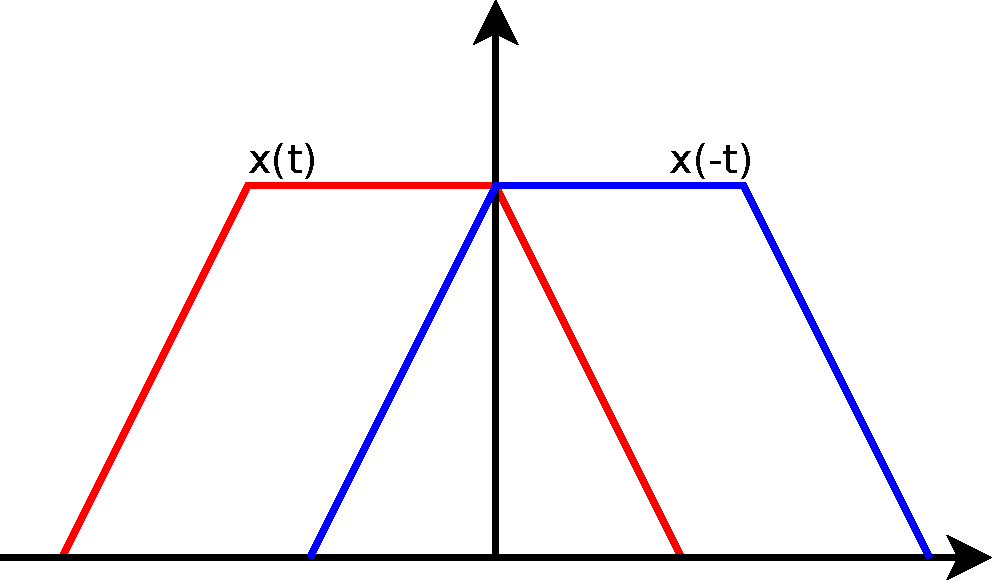
\includegraphics[width=50mm,keepaspectratio=true]{./Elektrotechnik/Bilder/argument.pdf}
  \end{center}
\end{multicols}

\begin{multicols}{2}
\subsubsection*{Nagation des Arguments \texorpdfstring{$t$}{} \\ sowie eine Verschiebung um \texorpdfstring{$t_0$}{}}
\begin{align*}
  &x_{neu}\left(t\right) = x_{alt}\left(t_0 - t\right) \\
  &\text{ mit } t_0 = const.\\
  &x_{neu}\left(t\right) = x_{alt}\left(\tau + 1/2 t_0\right)\\
  &x_{neu}\left(1/2 t_0 - \tau\right) = x_{alt}\left(\tau + 1/2 t_0\right)\\
\end{align*}
\vfill
\begin{center}
 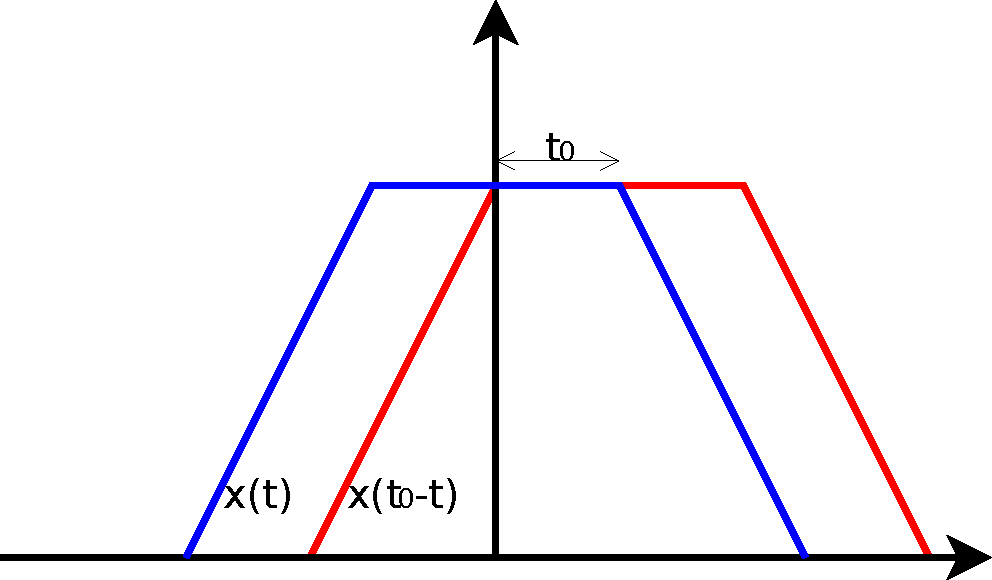
\includegraphics[width=50mm,keepaspectratio=true]{./Elektrotechnik/Bilder/argumentversch.pdf}
\end{center}

\end{multicols}
\begin{itemize}
 \item neue Zeitbasis \(\tau + 1/2 t_0\)
 \item gleiche Funktionswerte, gespiegelt an der Senkrechten von \(1/2 t_0\)
\end{itemize}

\subsubsection*{Skalierungsfaktor \texorpdfstring{$a \neq 0$}{}}
\index{Skalierungsfaktor}
\begin{multicols}{2}
\begin{align*}
  &x_{neu}\left(t\right) = x_{alt}\left(a \cdot t\right) \\
  &\text{ mit } a = const.\\
  &x_{neu}\left(t\right) = x_{alt}\left(\tau\right)\\
  &x_{neu}\left(\tau / a\right) = x_{alt}\left(\tau\right)
\end{align*}
\vfill
\begin{center}
 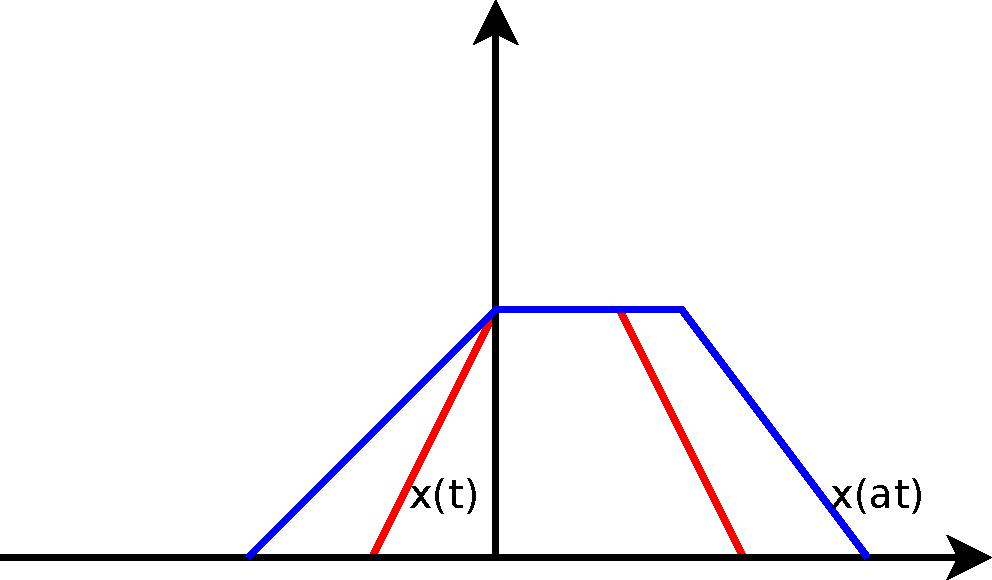
\includegraphics[width=50mm,keepaspectratio=true]{./Elektrotechnik/Bilder/skalierungsfaktor.pdf}
\end{center}

\end{multicols}
\begin{itemize}
 \item neue Zeitbasis \(\tau = a \cdot t\)
 \item gleiche Funktionswerte, wenn die Zeitbasis durch \(a\) geteilt wird
 \item \(a > 1\) Funktion wird gestaucht\\
       \(0 < a < 1\) Funktion wird gestreckt 
\end{itemize}

\subsection*{Einheitssprungfunktion}
\index{Einheitssprungfunktion}
\subsubsection*{angenäherte Einheitssprungfunktion
\texorpdfstring{$\tilde{\sigma}\left(t, \epsilon \right)$}{}}
\begin{multicols}{2}
 \begin{itemize}
  \item endlicher Geradenanstieg
  \item Endwert von 1
 \end{itemize}
\vfill
\begin{center}
 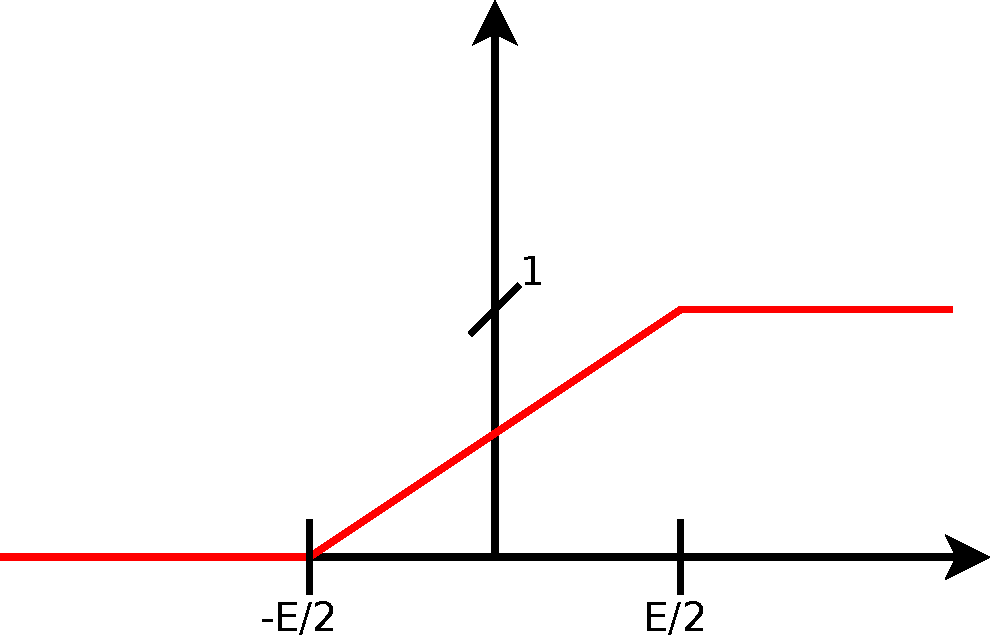
\includegraphics[width=50mm,keepaspectratio=true]{./Elektrotechnik/Bilder/einheitssprungang.pdf}
\end{center}
\vfill
\end{multicols}

\subsubsection*{Einheitsimpuls / Deltaimpuls
\index{Deltaimpuls}
\texorpdfstring{$\tilde{\delta}\left(t, \epsilon\right)$}{}}
\begin{multicols}{2}
\begin{itemize}
  \item Fläche des Impulses ist 1
  \item Impulshöhe und Breite variabel
\end{itemize}
\vfill
\begin{center}
	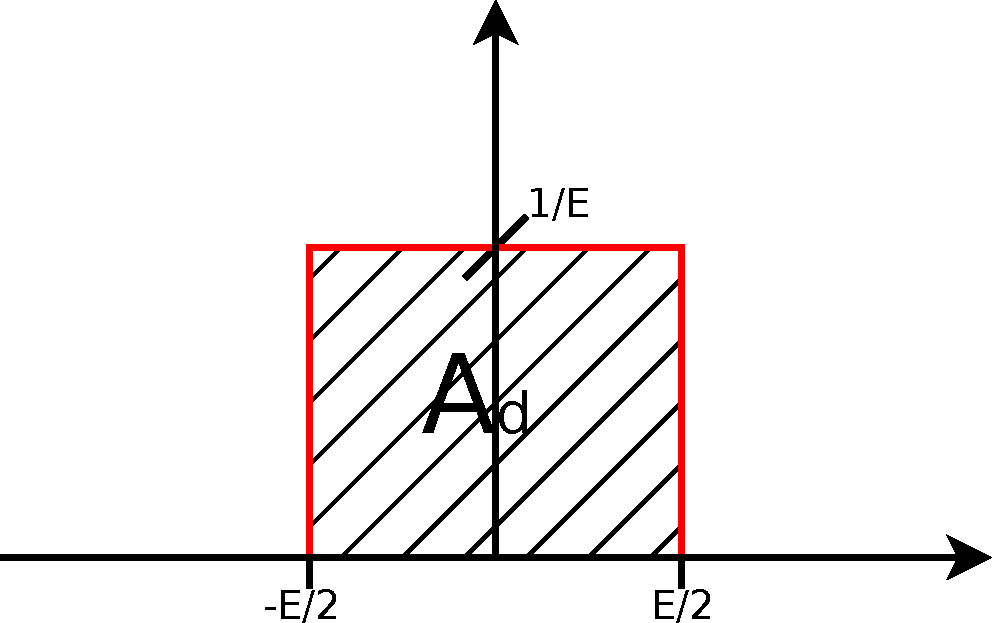
\includegraphics[width=50mm,keepaspectratio=true]{./Elektrotechnik/Bilder/einheitsimpuls.pdf}
\end{center}
\vfill
\end{multicols}


Mathematischer Zusammenhang:
\[
\tilde{\delta} \left(t, \epsilon \right) = \frac{d \tilde{\sigma} \left( t,
\epsilon \right)}{dt} \quad \leftrightarrow \quad \tilde{\sigma} \left( t,
\epsilon \right) = \int_{-\infty}^{t} \tilde{\delta} \left( t, \epsilon \right) dt
\]
Beim Grenzübergang \( \epsilon \rightarrow 0 \) ergibt die
Einheitssprungfunktion \( \sigma \left( t \right) \) bzw. deren Ableitung den
Deltaimpuls \( \delta \left( t \right) \).
\begin{multicols}{2}
\vfill
\[
\delta\left(t\right) = \frac{d \sigma \left(t\right)}{dt} = 
\begin{cases}
+ \infty \text{ für } t = 0 \\
\\
0 \text{ für } t \neq 0
\end{cases}
\]
\vfill
\[
\sigma \left(t\right) = \int_{-\infty}^{t} \delta \left(t\right)dt = 
\begin{cases}
1 \text{ für } t > 0\\
\frac{1}{2} \text{ für } t = 0\\
0 \text{ für } t < 0\\
\end{cases}
\]
\vfill
\end{multicols}

\subsection*{Zusammenhang zwischen Deltaimpuls, Einheitssprungfunktion und Einheitsanstiegsfunktion}
\index{Deltaimpuls}
\index{Einheitssprungfunktion}
\index{Einheitsanstiegsfunktion}
\begin{center}
	% Graphic for TeX using PGF
% Title: /home/Befedo/Documents/eclipse.workspace/Formelsammlung/Elektrotechnik/Bilder/zusammenhang.dia
% Creator: Dia v0.97
% CreationDate: Wed Feb 15 14:26:29 2012
% For: Befedo
% \usepackage{tikz}
% The following commands are not supported in PSTricks at present
% We define them conditionally, so when they are implemented,
% this pgf file will use them.
\ifx\du\undefined
  \newlength{\du}
\fi
\setlength{\du}{15\unitlength}
\begin{tikzpicture}
\pgftransformxscale{1.000000}
\pgftransformyscale{-1.000000}
\definecolor{dialinecolor}{rgb}{0.000000, 0.000000, 0.000000}
\pgfsetstrokecolor{dialinecolor}
\definecolor{dialinecolor}{rgb}{1.000000, 1.000000, 1.000000}
\pgfsetfillcolor{dialinecolor}
\pgfsetlinewidth{0.005000\du}
\pgfsetdash{}{0pt}
\pgfsetdash{}{0pt}
\pgfsetbuttcap
{
\definecolor{dialinecolor}{rgb}{0.000000, 0.000000, 0.000000}
\pgfsetfillcolor{dialinecolor}
% was here!!!
\pgfsetarrowsend{to}
\definecolor{dialinecolor}{rgb}{0.000000, 0.000000, 0.000000}
\pgfsetstrokecolor{dialinecolor}
\draw (1.000000\du,4.000000\du)--(23.000000\du,4.000000\du);
}
\pgfsetlinewidth{0.005000\du}
\pgfsetdash{}{0pt}
\pgfsetdash{}{0pt}
\pgfsetbuttcap
{
\definecolor{dialinecolor}{rgb}{0.000000, 0.000000, 0.000000}
\pgfsetfillcolor{dialinecolor}
% was here!!!
\pgfsetarrowsend{to}
\definecolor{dialinecolor}{rgb}{0.000000, 0.000000, 0.000000}
\pgfsetstrokecolor{dialinecolor}
\draw (5.000000\du,4.000000\du)--(5.000000\du,1.000000\du);
}
\pgfsetlinewidth{0.005000\du}
\pgfsetdash{}{0pt}
\pgfsetdash{}{0pt}
\pgfsetbuttcap
{
\definecolor{dialinecolor}{rgb}{0.000000, 0.000000, 0.000000}
\pgfsetfillcolor{dialinecolor}
% was here!!!
\pgfsetarrowsend{to}
\definecolor{dialinecolor}{rgb}{0.000000, 0.000000, 0.000000}
\pgfsetstrokecolor{dialinecolor}
\draw (12.000000\du,4.000000\du)--(12.000000\du,1.000000\du);
}
\pgfsetlinewidth{0.005000\du}
\pgfsetdash{}{0pt}
\pgfsetdash{}{0pt}
\pgfsetbuttcap
{
\definecolor{dialinecolor}{rgb}{0.000000, 0.000000, 0.000000}
\pgfsetfillcolor{dialinecolor}
% was here!!!
\pgfsetarrowsend{to}
\definecolor{dialinecolor}{rgb}{0.000000, 0.000000, 0.000000}
\pgfsetstrokecolor{dialinecolor}
\draw (19.000000\du,4.000000\du)--(19.000000\du,1.000000\du);
}
\pgfsetlinewidth{0.100000\du}
\pgfsetdash{}{0pt}
\pgfsetdash{}{0pt}
\pgfsetbuttcap
{
\definecolor{dialinecolor}{rgb}{1.000000, 0.000000, 0.000000}
\pgfsetfillcolor{dialinecolor}
% was here!!!
\definecolor{dialinecolor}{rgb}{1.000000, 0.000000, 0.000000}
\pgfsetstrokecolor{dialinecolor}
\draw (3.000000\du,4.000000\du)--(7.000000\du,4.000000\du);
}
\pgfsetlinewidth{0.100000\du}
\pgfsetdash{}{0pt}
\pgfsetdash{}{0pt}
\pgfsetbuttcap
{
\definecolor{dialinecolor}{rgb}{1.000000, 0.000000, 0.000000}
\pgfsetfillcolor{dialinecolor}
% was here!!!
\pgfsetarrowsend{to}
\definecolor{dialinecolor}{rgb}{1.000000, 0.000000, 0.000000}
\pgfsetstrokecolor{dialinecolor}
\draw (5.000000\du,4.000000\du)--(5.000000\du,2.000000\du);
}
\pgfsetlinewidth{0.100000\du}
\pgfsetdash{}{0pt}
\pgfsetdash{}{0pt}
\pgfsetbuttcap
{
\definecolor{dialinecolor}{rgb}{1.000000, 0.000000, 0.000000}
\pgfsetfillcolor{dialinecolor}
% was here!!!
\definecolor{dialinecolor}{rgb}{1.000000, 0.000000, 0.000000}
\pgfsetstrokecolor{dialinecolor}
\draw (12.000000\du,4.000000\du)--(10.000000\du,4.000000\du);
}
\pgfsetlinewidth{0.100000\du}
\pgfsetdash{}{0pt}
\pgfsetdash{}{0pt}
\pgfsetbuttcap
{
\definecolor{dialinecolor}{rgb}{1.000000, 0.000000, 0.000000}
\pgfsetfillcolor{dialinecolor}
% was here!!!
\definecolor{dialinecolor}{rgb}{1.000000, 0.000000, 0.000000}
\pgfsetstrokecolor{dialinecolor}
\draw (14.000000\du,2.000000\du)--(12.000000\du,2.000000\du);
}
\pgfsetlinewidth{0.100000\du}
\pgfsetdash{}{0pt}
\pgfsetdash{}{0pt}
\pgfsetbuttcap
{
\definecolor{dialinecolor}{rgb}{1.000000, 0.000000, 0.000000}
\pgfsetfillcolor{dialinecolor}
% was here!!!
\definecolor{dialinecolor}{rgb}{1.000000, 0.000000, 0.000000}
\pgfsetstrokecolor{dialinecolor}
\draw (17.000000\du,4.000000\du)--(19.000000\du,4.000000\du);
}
\pgfsetlinewidth{0.100000\du}
\pgfsetdash{}{0pt}
\pgfsetdash{}{0pt}
\pgfsetbuttcap
{
\definecolor{dialinecolor}{rgb}{1.000000, 0.000000, 0.000000}
\pgfsetfillcolor{dialinecolor}
% was here!!!
\definecolor{dialinecolor}{rgb}{1.000000, 0.000000, 0.000000}
\pgfsetstrokecolor{dialinecolor}
\draw (19.000000\du,4.000000\du)--(21.000000\du,2.000000\du);
}
\end{tikzpicture}

\end{center}

\begin{align*}
\delta \left( t \right) &= \frac{\mathrm{d} \sigma \left( t \right)}{\mathrm{dt}} =
\frac{\mathrm{d^2} \alpha \left( t \right)}{\mathrm{dt^2}} & \sigma \left( t \right) &=
\int\limits_{-\infty}^{t} \delta \left( t \right) \mathrm{dt} =
\frac{\mathrm{d} \alpha \left( t \right)}{\mathrm{dt}}
\end{align*}

\[
\alpha \left( t \right) = 
\begin{cases}
	t \text{ für } t > 0
	\\
	\\
	0 \text{ für } t \leq 0
\end{cases}
= \int\limits_{-\infty}^{t} \sigma \left( t \right) \mathrm{dt}
= \int\limits_{-\infty}^{t} \int\limits_{-\infty}^{t} \delta \left( t \right) \mathrm{dt}
\]

\subsection*{zeitliche Verschiebung und Wichtung}

\subsubsection*{Deltaimpuls}
	\begin{multicols}{2}
		\vfill
		\begin{align*}
			x \left( t \right) &= A_x \cdot \delta \left( t - t_0 \right) \\
			\left[ x\left(t\right) \right] &= \left[ A_x \right] \cdot \left[ \delta\left( t \right) \right]
		\end{align*}
		\vspace{20mm}
		\vfill
		% Graphic for TeX using PGF
% Title: /home/Befedo/Documents/eclipse.workspace/Formelsammlung/Elektrotechnik/Bilder/delta.dia
% Creator: Dia v0.97
% CreationDate: Wed Feb 15 15:27:30 2012
% For: Befedo
% \usepackage{tikz}
% The following commands are not supported in PSTricks at present
% We define them conditionally, so when they are implemented,
% this pgf file will use them.
\ifx\du\undefined
  \newlength{\du}
\fi
\setlength{\du}{15\unitlength}
\begin{tikzpicture}
\pgftransformxscale{1.000000}
\pgftransformyscale{-1.000000}
\definecolor{dialinecolor}{rgb}{0.000000, 0.000000, 0.000000}
\pgfsetstrokecolor{dialinecolor}
\definecolor{dialinecolor}{rgb}{1.000000, 1.000000, 1.000000}
\pgfsetfillcolor{dialinecolor}
\pgfsetlinewidth{0.100000\du}
\pgfsetdash{}{0pt}
\pgfsetdash{}{0pt}
\pgfsetbuttcap
{
\definecolor{dialinecolor}{rgb}{0.000000, 0.000000, 0.000000}
\pgfsetfillcolor{dialinecolor}
% was here!!!
\definecolor{dialinecolor}{rgb}{0.000000, 0.000000, 0.000000}
\pgfsetstrokecolor{dialinecolor}
\draw (13.500000\du,3.500000\du)--(14.500000\du,2.500000\du);
}
% setfont left to latex
\definecolor{dialinecolor}{rgb}{0.000000, 0.000000, 0.000000}
\pgfsetstrokecolor{dialinecolor}
\node[anchor=west] at (14.500000\du,2.500000\du){};
\pgfsetlinewidth{0.100000\du}
\pgfsetdash{}{0pt}
\pgfsetdash{}{0pt}
\pgfsetbuttcap
{
\definecolor{dialinecolor}{rgb}{0.000000, 0.000000, 0.000000}
\pgfsetfillcolor{dialinecolor}
% was here!!!
\pgfsetarrowsend{stealth}
\definecolor{dialinecolor}{rgb}{0.000000, 0.000000, 0.000000}
\pgfsetstrokecolor{dialinecolor}
\draw (14.000000\du,5.500000\du)--(14.000000\du,1.000000\du);
}
\pgfsetlinewidth{0.100000\du}
\pgfsetdash{}{0pt}
\pgfsetdash{}{0pt}
\pgfsetbuttcap
{
\definecolor{dialinecolor}{rgb}{0.000000, 0.000000, 0.000000}
\pgfsetfillcolor{dialinecolor}
% was here!!!
\pgfsetarrowsend{stealth}
\definecolor{dialinecolor}{rgb}{0.000000, 0.000000, 0.000000}
\pgfsetstrokecolor{dialinecolor}
\draw (9.500000\du,5.500000\du)--(18.500000\du,5.500000\du);
}
\pgfsetlinewidth{0.150000\du}
\pgfsetdash{}{0pt}
\pgfsetdash{}{0pt}
\pgfsetbuttcap
{
\definecolor{dialinecolor}{rgb}{1.000000, 0.000000, 0.000000}
\pgfsetfillcolor{dialinecolor}
% was here!!!
\pgfsetarrowsend{to}
\definecolor{dialinecolor}{rgb}{1.000000, 0.000000, 0.000000}
\pgfsetstrokecolor{dialinecolor}
\draw (16.000000\du,5.500000\du)--(16.000000\du,3.000000\du);
}
% setfont left to latex
\definecolor{dialinecolor}{rgb}{0.000000, 0.000000, 0.000000}
\pgfsetstrokecolor{dialinecolor}
\node[anchor=west] at (14.500000\du,2.500000\du){Ax};
\pgfsetlinewidth{0.100000\du}
\pgfsetdash{}{0pt}
\pgfsetdash{}{0pt}
\pgfsetbuttcap
{
\definecolor{dialinecolor}{rgb}{0.000000, 0.000000, 0.000000}
\pgfsetfillcolor{dialinecolor}
% was here!!!
\definecolor{dialinecolor}{rgb}{0.000000, 0.000000, 0.000000}
\pgfsetstrokecolor{dialinecolor}
\draw (16.000000\du,5.000000\du)--(16.000000\du,6.000000\du);
}
% setfont left to latex
\definecolor{dialinecolor}{rgb}{0.000000, 0.000000, 0.000000}
\pgfsetstrokecolor{dialinecolor}
\node[anchor=west] at (16.200000\du,6.400000\du){t};
% setfont left to latex
\definecolor{dialinecolor}{rgb}{0.000000, 0.000000, 0.000000}
\pgfsetstrokecolor{dialinecolor}
\node[anchor=west] at (16.500000\du,6.500000\du){0};
\end{tikzpicture}

		\vfill
	\end{multicols}
	
\subsubsection*{Einheitssprung}
	\begin{multicols}{2}
		\vfill
		\begin{align*}
			x\left( t \right) &= X_0 \cdot \sigma \left( t - t_0 \right) \\
			\left[ x\left( t \right) \right] &= \left[ X_0 \right]
		\end{align*}
		\vspace{20mm}
		\vfill
		% Graphic for TeX using PGF
% Title: /home/Befedo/Documents/eclipse.workspace/Formelsammlung/Elektrotechnik/Bilder/einheitssprung.dia
% Creator: Dia v0.97
% CreationDate: Wed Feb 15 22:13:28 2012
% For: Befedo
% \usepackage{tikz}
% The following commands are not supported in PSTricks at present
% We define them conditionally, so when they are implemented,
% this pgf file will use them.
\ifx\du\undefined
  \newlength{\du}
\fi
\setlength{\du}{15\unitlength}
\begin{tikzpicture}
\pgftransformxscale{1.000000}
\pgftransformyscale{-1.000000}
\definecolor{dialinecolor}{rgb}{0.000000, 0.000000, 0.000000}
\pgfsetstrokecolor{dialinecolor}
\definecolor{dialinecolor}{rgb}{1.000000, 1.000000, 1.000000}
\pgfsetfillcolor{dialinecolor}
\pgfsetlinewidth{0.100000\du}
\pgfsetdash{}{0pt}
\pgfsetdash{}{0pt}
\pgfsetbuttcap
{
\definecolor{dialinecolor}{rgb}{0.000000, 0.000000, 0.000000}
\pgfsetfillcolor{dialinecolor}
% was here!!!
\definecolor{dialinecolor}{rgb}{0.000000, 0.000000, 0.000000}
\pgfsetstrokecolor{dialinecolor}
\draw (9.000000\du,3.500000\du)--(10.000000\du,2.500000\du);
}
% setfont left to latex
\definecolor{dialinecolor}{rgb}{0.000000, 0.000000, 0.000000}
\pgfsetstrokecolor{dialinecolor}
\node[anchor=west] at (14.500000\du,2.500000\du){};
\pgfsetlinewidth{0.100000\du}
\pgfsetdash{}{0pt}
\pgfsetdash{}{0pt}
\pgfsetbuttcap
{
\definecolor{dialinecolor}{rgb}{0.000000, 0.000000, 0.000000}
\pgfsetfillcolor{dialinecolor}
% was here!!!
\pgfsetarrowsend{stealth}
\definecolor{dialinecolor}{rgb}{0.000000, 0.000000, 0.000000}
\pgfsetstrokecolor{dialinecolor}
\draw (9.500000\du,5.500000\du)--(9.500000\du,1.000000\du);
}
\pgfsetlinewidth{0.100000\du}
\pgfsetdash{}{0pt}
\pgfsetdash{}{0pt}
\pgfsetbuttcap
{
\definecolor{dialinecolor}{rgb}{0.000000, 0.000000, 0.000000}
\pgfsetfillcolor{dialinecolor}
% was here!!!
\pgfsetarrowsend{stealth}
\definecolor{dialinecolor}{rgb}{0.000000, 0.000000, 0.000000}
\pgfsetstrokecolor{dialinecolor}
\draw (9.500000\du,5.500000\du)--(18.500000\du,5.500000\du);
}
% setfont left to latex
\definecolor{dialinecolor}{rgb}{0.000000, 0.000000, 0.000000}
\pgfsetstrokecolor{dialinecolor}
\node[anchor=west] at (10.000000\du,2.500000\du){X};
\pgfsetlinewidth{0.100000\du}
\pgfsetdash{}{0pt}
\pgfsetdash{}{0pt}
\pgfsetbuttcap
{
\definecolor{dialinecolor}{rgb}{0.000000, 0.000000, 0.000000}
\pgfsetfillcolor{dialinecolor}
% was here!!!
\definecolor{dialinecolor}{rgb}{0.000000, 0.000000, 0.000000}
\pgfsetstrokecolor{dialinecolor}
\draw (14.000000\du,5.000000\du)--(14.000000\du,6.000000\du);
}
% setfont left to latex
\definecolor{dialinecolor}{rgb}{0.000000, 0.000000, 0.000000}
\pgfsetstrokecolor{dialinecolor}
\node[anchor=west] at (14.000000\du,6.500000\du){t};
% setfont left to latex
\definecolor{dialinecolor}{rgb}{0.000000, 0.000000, 0.000000}
\pgfsetstrokecolor{dialinecolor}
\node[anchor=west] at (14.300000\du,6.600000\du){0};
\pgfsetlinewidth{0.150000\du}
\pgfsetdash{}{0pt}
\pgfsetdash{}{0pt}
\pgfsetbuttcap
{
\definecolor{dialinecolor}{rgb}{1.000000, 0.000000, 0.000000}
\pgfsetfillcolor{dialinecolor}
% was here!!!
\definecolor{dialinecolor}{rgb}{1.000000, 0.000000, 0.000000}
\pgfsetstrokecolor{dialinecolor}
\draw (9.500000\du,5.500000\du)--(14.000000\du,5.500000\du);
}
\pgfsetlinewidth{0.150000\du}
\pgfsetdash{}{0pt}
\pgfsetdash{}{0pt}
\pgfsetbuttcap
{
\definecolor{dialinecolor}{rgb}{1.000000, 0.000000, 0.000000}
\pgfsetfillcolor{dialinecolor}
% was here!!!
\definecolor{dialinecolor}{rgb}{1.000000, 0.000000, 0.000000}
\pgfsetstrokecolor{dialinecolor}
\draw (14.000000\du,3.000000\du)--(17.500000\du,3.000000\du);
}
% setfont left to latex
\definecolor{dialinecolor}{rgb}{0.000000, 0.000000, 0.000000}
\pgfsetstrokecolor{dialinecolor}
\node[anchor=west] at (10.435781\du,2.493530\du){0};
\end{tikzpicture}

		\vfill
	\end{multicols}
	
\subsubsection*{Einheitsanstiegsfunktion}
	\begin{multicols}{2}
		\vfill
		\begin{align*}
			x \left( t \right) &= m \cdot \alpha \left( t - t_0 \right) \\
			\left[ x \left( t \right) \right] &= \left[ m \right] \cdot \left[ \alpha \left(t\right) \right]
		\end{align*}
		\vspace{20mm}
		\vfill
		% Graphic for TeX using PGF
% Title: /home/Befedo/Documents/eclipse.workspace/Formelsammlung/Elektrotechnik/Bilder/einheitsanstieg.dia
% Creator: Dia v0.97
% CreationDate: Wed Feb 15 16:40:58 2012
% For: Befedo
% \usepackage{tikz}
% The following commands are not supported in PSTricks at present
% We define them conditionally, so when they are implemented,
% this pgf file will use them.
\ifx\du\undefined
  \newlength{\du}
\fi
\setlength{\du}{15\unitlength}
\begin{tikzpicture}
\pgftransformxscale{1.000000}
\pgftransformyscale{-1.000000}
\definecolor{dialinecolor}{rgb}{0.000000, 0.000000, 0.000000}
\pgfsetstrokecolor{dialinecolor}
\definecolor{dialinecolor}{rgb}{1.000000, 1.000000, 1.000000}
\pgfsetfillcolor{dialinecolor}
% setfont left to latex
\definecolor{dialinecolor}{rgb}{0.000000, 0.000000, 0.000000}
\pgfsetstrokecolor{dialinecolor}
\node[anchor=west] at (14.500000\du,2.500000\du){};
\pgfsetlinewidth{0.100000\du}
\pgfsetdash{}{0pt}
\pgfsetdash{}{0pt}
\pgfsetbuttcap
{
\definecolor{dialinecolor}{rgb}{0.000000, 0.000000, 0.000000}
\pgfsetfillcolor{dialinecolor}
% was here!!!
\pgfsetarrowsend{stealth}
\definecolor{dialinecolor}{rgb}{0.000000, 0.000000, 0.000000}
\pgfsetstrokecolor{dialinecolor}
\draw (9.500000\du,5.500000\du)--(9.500000\du,1.000000\du);
}
\pgfsetlinewidth{0.100000\du}
\pgfsetdash{}{0pt}
\pgfsetdash{}{0pt}
\pgfsetbuttcap
{
\definecolor{dialinecolor}{rgb}{0.000000, 0.000000, 0.000000}
\pgfsetfillcolor{dialinecolor}
% was here!!!
\pgfsetarrowsend{stealth}
\definecolor{dialinecolor}{rgb}{0.000000, 0.000000, 0.000000}
\pgfsetstrokecolor{dialinecolor}
\draw (9.500000\du,5.500000\du)--(18.500000\du,5.500000\du);
}
\pgfsetlinewidth{0.100000\du}
\pgfsetdash{}{0pt}
\pgfsetdash{}{0pt}
\pgfsetbuttcap
{
\definecolor{dialinecolor}{rgb}{0.000000, 0.000000, 0.000000}
\pgfsetfillcolor{dialinecolor}
% was here!!!
\definecolor{dialinecolor}{rgb}{0.000000, 0.000000, 0.000000}
\pgfsetstrokecolor{dialinecolor}
\draw (14.000000\du,5.000000\du)--(14.000000\du,6.000000\du);
}
% setfont left to latex
\definecolor{dialinecolor}{rgb}{0.000000, 0.000000, 0.000000}
\pgfsetstrokecolor{dialinecolor}
\node[anchor=west] at (14.000000\du,6.500000\du){t};
% setfont left to latex
\definecolor{dialinecolor}{rgb}{0.000000, 0.000000, 0.000000}
\pgfsetstrokecolor{dialinecolor}
\node[anchor=west] at (14.300000\du,6.600000\du){0};
\pgfsetlinewidth{0.150000\du}
\pgfsetdash{}{0pt}
\pgfsetdash{}{0pt}
\pgfsetbuttcap
{
\definecolor{dialinecolor}{rgb}{1.000000, 0.000000, 0.000000}
\pgfsetfillcolor{dialinecolor}
% was here!!!
\definecolor{dialinecolor}{rgb}{1.000000, 0.000000, 0.000000}
\pgfsetstrokecolor{dialinecolor}
\draw (9.500000\du,5.500000\du)--(14.000000\du,5.500000\du);
}
\pgfsetlinewidth{0.150000\du}
\pgfsetdash{}{0pt}
\pgfsetdash{}{0pt}
\pgfsetbuttcap
{
\definecolor{dialinecolor}{rgb}{1.000000, 0.000000, 0.000000}
\pgfsetfillcolor{dialinecolor}
% was here!!!
\definecolor{dialinecolor}{rgb}{1.000000, 0.000000, 0.000000}
\pgfsetstrokecolor{dialinecolor}
\draw (14.000000\du,5.500000\du)--(17.500000\du,2.500000\du);
}
\end{tikzpicture}

		\vfill
	\end{multicols}
	
\newpage
\section{Signale}
\index{Signale!Definition}
\textbf{Definition:}
Ein Signal ist eine zeitlich und / oder örtlich veränderliche Größe (physikalisch).
Die Veränderung dieser physikalischen Größe, sagt nichts über Ihren Informationsgehalt aus.
	
\begin{center}
	% Graphic for TeX using PGF
% Title: /home/Befedo/Documents/eclipse.workspace/Formelsammlung/Elektrotechnik/Bilder/signalstatistik.dia
% Creator: Dia v0.97
% CreationDate: Wed Feb 15 23:22:16 2012
% For: Befedo
% \usepackage{tikz}
% The following commands are not supported in PSTricks at present
% We define them conditionally, so when they are implemented,
% this pgf file will use them.
\ifx\du\undefined
  \newlength{\du}
\fi
\setlength{\du}{15\unitlength}
\begin{tikzpicture}
\pgftransformxscale{1.000000}
\pgftransformyscale{-1.000000}
\definecolor{dialinecolor}{rgb}{0.000000, 0.000000, 0.000000}
\pgfsetstrokecolor{dialinecolor}
\definecolor{dialinecolor}{rgb}{1.000000, 1.000000, 1.000000}
\pgfsetfillcolor{dialinecolor}
\pgfsetlinewidth{0.100000\du}
\pgfsetdash{}{0pt}
{\pgfsetcornersarced{\pgfpoint{0.500000\du}{0.500000\du}}\definecolor{dialinecolor}{rgb}{1.000000, 1.000000, 1.000000}
\pgfsetfillcolor{dialinecolor}
\fill (9.500000\du,0.500000\du)--(9.500000\du,2.300000\du)--(13.500000\du,2.300000\du)--(13.500000\du,0.500000\du)--cycle;
}{\pgfsetcornersarced{\pgfpoint{0.500000\du}{0.500000\du}}\definecolor{dialinecolor}{rgb}{0.000000, 0.000000, 0.000000}
\pgfsetstrokecolor{dialinecolor}
\draw (9.500000\du,0.500000\du)--(9.500000\du,2.300000\du)--(13.500000\du,2.300000\du)--(13.500000\du,0.500000\du)--cycle;
}% setfont left to latex
\definecolor{dialinecolor}{rgb}{0.000000, 0.000000, 0.000000}
\pgfsetstrokecolor{dialinecolor}
\node at (11.500000\du,1.595000\du){Signal};
\pgfsetlinewidth{0.100000\du}
\pgfsetdash{}{0pt}
{\pgfsetcornersarced{\pgfpoint{0.500000\du}{0.500000\du}}\definecolor{dialinecolor}{rgb}{1.000000, 1.000000, 1.000000}
\pgfsetfillcolor{dialinecolor}
\fill (2.500000\du,3.500000\du)--(2.500000\du,5.300000\du)--(7.830000\du,5.300000\du)--(7.830000\du,3.500000\du)--cycle;
}{\pgfsetcornersarced{\pgfpoint{0.500000\du}{0.500000\du}}\definecolor{dialinecolor}{rgb}{0.000000, 0.000000, 0.000000}
\pgfsetstrokecolor{dialinecolor}
\draw (2.500000\du,3.500000\du)--(2.500000\du,5.300000\du)--(7.830000\du,5.300000\du)--(7.830000\du,3.500000\du)--cycle;
}% setfont left to latex
\definecolor{dialinecolor}{rgb}{0.000000, 0.000000, 0.000000}
\pgfsetstrokecolor{dialinecolor}
\node at (5.165000\du,4.595000\du){Energiesignal};
\pgfsetlinewidth{0.100000\du}
\pgfsetdash{}{0pt}
{\pgfsetcornersarced{\pgfpoint{0.500000\du}{0.500000\du}}\definecolor{dialinecolor}{rgb}{1.000000, 1.000000, 1.000000}
\pgfsetfillcolor{dialinecolor}
\fill (15.000000\du,3.500000\du)--(15.000000\du,5.300000\du)--(20.612500\du,5.300000\du)--(20.612500\du,3.500000\du)--cycle;
}{\pgfsetcornersarced{\pgfpoint{0.500000\du}{0.500000\du}}\definecolor{dialinecolor}{rgb}{0.000000, 0.000000, 0.000000}
\pgfsetstrokecolor{dialinecolor}
\draw (15.000000\du,3.500000\du)--(15.000000\du,5.300000\du)--(20.612500\du,5.300000\du)--(20.612500\du,3.500000\du)--cycle;
}% setfont left to latex
\definecolor{dialinecolor}{rgb}{0.000000, 0.000000, 0.000000}
\pgfsetstrokecolor{dialinecolor}
\node at (17.806250\du,4.595000\du){Leistungsignal};
\pgfsetlinewidth{0.100000\du}
\pgfsetdash{}{0pt}
\pgfsetdash{}{0pt}
\pgfsetbuttcap
{
\definecolor{dialinecolor}{rgb}{0.000000, 0.000000, 0.000000}
\pgfsetfillcolor{dialinecolor}
% was here!!!
\pgfsetarrowsend{stealth}
\definecolor{dialinecolor}{rgb}{0.000000, 0.000000, 0.000000}
\pgfsetstrokecolor{dialinecolor}
\draw (9.500000\du,2.300000\du)--(8.000000\du,3.500000\du);
}
\pgfsetlinewidth{0.100000\du}
\pgfsetdash{}{0pt}
\pgfsetdash{}{0pt}
\pgfsetbuttcap
{
\definecolor{dialinecolor}{rgb}{0.000000, 0.000000, 0.000000}
\pgfsetfillcolor{dialinecolor}
% was here!!!
\pgfsetarrowsend{stealth}
\definecolor{dialinecolor}{rgb}{0.000000, 0.000000, 0.000000}
\pgfsetstrokecolor{dialinecolor}
\draw (13.500000\du,2.300000\du)--(15.000000\du,3.500000\du);
}
\pgfsetlinewidth{0.100000\du}
\pgfsetdash{}{0pt}
\pgfsetdash{}{0pt}
\pgfsetbuttcap
{
\definecolor{dialinecolor}{rgb}{0.000000, 0.000000, 0.000000}
\pgfsetfillcolor{dialinecolor}
% was here!!!
\pgfsetarrowsend{stealth}
\definecolor{dialinecolor}{rgb}{0.000000, 0.000000, 0.000000}
\pgfsetstrokecolor{dialinecolor}
\draw (2.500000\du,5.300000\du)--(1.500000\du,7.000000\du);
}
\pgfsetlinewidth{0.100000\du}
\pgfsetdash{}{0pt}
\pgfsetdash{}{0pt}
\pgfsetbuttcap
{
\definecolor{dialinecolor}{rgb}{0.000000, 0.000000, 0.000000}
\pgfsetfillcolor{dialinecolor}
% was here!!!
\pgfsetarrowsend{stealth}
\definecolor{dialinecolor}{rgb}{0.000000, 0.000000, 0.000000}
\pgfsetstrokecolor{dialinecolor}
\draw (5.165000\du,5.300000\du)--(5.500000\du,6.975000\du);
}
\pgfsetlinewidth{0.100000\du}
\pgfsetdash{}{0pt}
\pgfsetdash{}{0pt}
\pgfsetbuttcap
{
\definecolor{dialinecolor}{rgb}{0.000000, 0.000000, 0.000000}
\pgfsetfillcolor{dialinecolor}
% was here!!!
\pgfsetarrowsend{stealth}
\definecolor{dialinecolor}{rgb}{0.000000, 0.000000, 0.000000}
\pgfsetstrokecolor{dialinecolor}
\draw (7.830000\du,5.300000\du)--(10.000000\du,7.000000\du);
}
\pgfsetlinewidth{0.100000\du}
\pgfsetdash{}{0pt}
\pgfsetdash{}{0pt}
\pgfsetbuttcap
{
\definecolor{dialinecolor}{rgb}{0.000000, 0.000000, 0.000000}
\pgfsetfillcolor{dialinecolor}
% was here!!!
\pgfsetarrowsend{stealth}
\definecolor{dialinecolor}{rgb}{0.000000, 0.000000, 0.000000}
\pgfsetstrokecolor{dialinecolor}
\draw (17.806250\du,5.300000\du)--(18.000000\du,7.000000\du);
}
\pgfsetlinewidth{0.100000\du}
\pgfsetdash{}{0pt}
\pgfsetdash{}{0pt}
\pgfsetmiterjoin
\definecolor{dialinecolor}{rgb}{1.000000, 1.000000, 1.000000}
\pgfsetfillcolor{dialinecolor}
\fill (0.000000\du,7.000000\du)--(0.000000\du,8.500000\du)--(3.000000\du,8.500000\du)--(3.000000\du,7.000000\du)--cycle;
\definecolor{dialinecolor}{rgb}{0.000000, 0.000000, 0.000000}
\pgfsetstrokecolor{dialinecolor}
\draw (0.000000\du,7.000000\du)--(0.000000\du,8.500000\du)--(3.000000\du,8.500000\du)--(3.000000\du,7.000000\du)--cycle;
% setfont left to latex
\definecolor{dialinecolor}{rgb}{0.000000, 0.000000, 0.000000}
\pgfsetstrokecolor{dialinecolor}
\node at (1.500000\du,7.500000\du){zeitlich};
% setfont left to latex
\definecolor{dialinecolor}{rgb}{0.000000, 0.000000, 0.000000}
\pgfsetstrokecolor{dialinecolor}
\node at (1.500000\du,8.088433\du){begrenzt};
\pgfsetlinewidth{0.100000\du}
\pgfsetdash{}{0pt}
\pgfsetdash{}{0pt}
\pgfsetmiterjoin
\definecolor{dialinecolor}{rgb}{1.000000, 1.000000, 1.000000}
\pgfsetfillcolor{dialinecolor}
\fill (3.500000\du,6.975000\du)--(3.500000\du,8.475000\du)--(7.500000\du,8.475000\du)--(7.500000\du,6.975000\du)--cycle;
\definecolor{dialinecolor}{rgb}{0.000000, 0.000000, 0.000000}
\pgfsetstrokecolor{dialinecolor}
\draw (3.500000\du,6.975000\du)--(3.500000\du,8.475000\du)--(7.500000\du,8.475000\du)--(7.500000\du,6.975000\du)--cycle;
% setfont left to latex
\definecolor{dialinecolor}{rgb}{0.000000, 0.000000, 0.000000}
\pgfsetstrokecolor{dialinecolor}
\node at (5.500000\du,7.500000\du){abklingende};
% setfont left to latex
\definecolor{dialinecolor}{rgb}{0.000000, 0.000000, 0.000000}
\pgfsetstrokecolor{dialinecolor}
\node at (5.500000\du,8.088433\du){Amplitude};
\pgfsetlinewidth{0.100000\du}
\pgfsetdash{}{0pt}
\pgfsetdash{}{0pt}
\pgfsetmiterjoin
\definecolor{dialinecolor}{rgb}{1.000000, 1.000000, 1.000000}
\pgfsetfillcolor{dialinecolor}
\fill (8.000000\du,7.000000\du)--(8.000000\du,8.500000\du)--(12.000000\du,8.500000\du)--(12.000000\du,7.000000\du)--cycle;
\definecolor{dialinecolor}{rgb}{0.000000, 0.000000, 0.000000}
\pgfsetstrokecolor{dialinecolor}
\draw (8.000000\du,7.000000\du)--(8.000000\du,8.500000\du)--(12.000000\du,8.500000\du)--(12.000000\du,7.000000\du)--cycle;
% setfont left to latex
\definecolor{dialinecolor}{rgb}{0.000000, 0.000000, 0.000000}
\pgfsetstrokecolor{dialinecolor}
\node at (10.000000\du,7.500000\du){sehr große};
% setfont left to latex
\definecolor{dialinecolor}{rgb}{0.000000, 0.000000, 0.000000}
\pgfsetstrokecolor{dialinecolor}
\node at (10.000000\du,8.088433\du){Pausenzeit};
\pgfsetlinewidth{0.100000\du}
\pgfsetdash{}{0pt}
\pgfsetdash{}{0pt}
\pgfsetmiterjoin
\definecolor{dialinecolor}{rgb}{1.000000, 1.000000, 1.000000}
\pgfsetfillcolor{dialinecolor}
\fill (16.000000\du,7.000000\du)--(16.000000\du,8.500000\du)--(20.000000\du,8.500000\du)--(20.000000\du,7.000000\du)--cycle;
\definecolor{dialinecolor}{rgb}{0.000000, 0.000000, 0.000000}
\pgfsetstrokecolor{dialinecolor}
\draw (16.000000\du,7.000000\du)--(16.000000\du,8.500000\du)--(20.000000\du,8.500000\du)--(20.000000\du,7.000000\du)--cycle;
% setfont left to latex
\definecolor{dialinecolor}{rgb}{0.000000, 0.000000, 0.000000}
\pgfsetstrokecolor{dialinecolor}
\node at (18.000000\du,7.500000\du){zeitlich};
% setfont left to latex
\definecolor{dialinecolor}{rgb}{0.000000, 0.000000, 0.000000}
\pgfsetstrokecolor{dialinecolor}
\node at (18.000000\du,8.088433\du){unbegrenzt};
% setfont left to latex
\definecolor{dialinecolor}{rgb}{0.000000, 0.000000, 0.000000}
\pgfsetstrokecolor{dialinecolor}
\node[anchor=west] at (0.500000\du,9.000000\du){-rect};
% setfont left to latex
\definecolor{dialinecolor}{rgb}{0.000000, 0.000000, 0.000000}
\pgfsetstrokecolor{dialinecolor}
\node[anchor=west] at (0.500000\du,9.447322\du){};
% setfont left to latex
\definecolor{dialinecolor}{rgb}{0.000000, 0.000000, 0.000000}
\pgfsetstrokecolor{dialinecolor}
\node[anchor=west] at (0.500000\du,9.894644\du){-Delta};
% setfont left to latex
\definecolor{dialinecolor}{rgb}{0.000000, 0.000000, 0.000000}
\pgfsetstrokecolor{dialinecolor}
\node[anchor=west] at (4.000000\du,9.000000\du){-exp-F.};
% setfont left to latex
\definecolor{dialinecolor}{rgb}{0.000000, 0.000000, 0.000000}
\pgfsetstrokecolor{dialinecolor}
\node[anchor=west] at (8.500000\du,9.000000\du){-Burst};
% setfont left to latex
\definecolor{dialinecolor}{rgb}{0.000000, 0.000000, 0.000000}
\pgfsetstrokecolor{dialinecolor}
\node[anchor=west] at (8.500000\du,9.447322\du){};
% setfont left to latex
\definecolor{dialinecolor}{rgb}{0.000000, 0.000000, 0.000000}
\pgfsetstrokecolor{dialinecolor}
\node[anchor=west] at (8.500000\du,9.894644\du){-Ethernet Paket};
% setfont left to latex
\definecolor{dialinecolor}{rgb}{0.000000, 0.000000, 0.000000}
\pgfsetstrokecolor{dialinecolor}
\node[anchor=west] at (16.500000\du,9.000000\du){-Sinus};
% setfont left to latex
\definecolor{dialinecolor}{rgb}{0.000000, 0.000000, 0.000000}
\pgfsetstrokecolor{dialinecolor}
\node[anchor=west] at (16.500000\du,9.447322\du){};
% setfont left to latex
\definecolor{dialinecolor}{rgb}{0.000000, 0.000000, 0.000000}
\pgfsetstrokecolor{dialinecolor}
\node[anchor=west] at (16.500000\du,9.894644\du){-Rauschen};
\end{tikzpicture}

\end{center}

\subsection*{Energiewandlung}
\index{Signale!Energiewandlung}
\begin{align*}
	E_R &= \int\limits_{-\infty}^{\infty} u \left( t \right) \cdot i \left( t \right) \mathrm{dt} &
	\left[ E_R \right] &= V \cdot A \cdot s = Ws 
	\\
	\text{mit } i \left( t \right) &= \frac{u \left( t \right)}{R} \text{ folgt}
	\\
	E_R &= \frac{1}{R}\int\limits_{-\infty}^{\infty}u^2 \left( t \right) \mathrm{dt}  
\end{align*}

\subsection*{Momentanleistung \texorpdfstring{$P_r\left(t_1\right)$}}
\index{Signale!Momentanleistung}
\begin{align*}
	P_R \left(t_1\right) &= u\left(t_1\right) \cdot i\left(t_1\right) &
	&\left[P_R\left(t_1\right)\right] = W
	\\
	P_R &= U_0 \cdot I_0 = \frac{U_0^2}{R} & &\text{ bei Gleichleistung}	
\end{align*}

\subsection*{Mittlere Leistung \texorpdfstring{$P_R$}}
\index{Signale!Mittlere Leistung}
\begin{align*}
	P_R &= \lim\limits_{T \to \infty} \frac{1}{T} \int\limits_{t_1}^{t_1 + T} u\left(t\right) \cdot
	i\left(t\right) \mathrm{dt} & \left[P_R\right] &= W
	\\
	    &= \frac{1}{R} \cdot \lim\limits_{T \to \infty} \frac{1}{T} \int\limits_{t_1}^{t_1 + T} u^2
		\left(t\right) \mathrm{dt}
	\\
	&\textbf{Spezialfall: } \text{Periodische Signalverläufe}
	\\
		&= \frac{1}{n \cdot t_P} \int\limits_{t_1}^{t_1 + n\cdot t_P} u_P \left(t\right) \cdot
		i_P\left(t\right) \mathrm{dt} = \frac{1}{R \cdot n \cdot t_P} \int\limits_{t_1}^{t_1 + n \cdot
		t_P} u_P^2 \left(t\right) \mathrm{dt}
\end{align*}
\[T \text{: Betrachtungszeit, Meßdauer } t_1 \text{: Startzeitpunkt } t_P \text{: Periodendauer } R
= const.\]

\subsection*{Signalenergie / Impulsenergie / Impulsmoment 2. Ordnung \texorpdfstring{$E_U$}}
\index{Signalenergie}
\index{Impulsenergie}
\index{Impulsmoment 2. Ordnung}
Nur für Energiesignale sinnvoll.
\begin{align*}
	E_U &= {m_i}_2 = \int\limits_{-\infty}^{\infty}u^2\left(t\right) \mathrm{dt} & \left[E_U\right] =
	{V^2}s
\end{align*}

Zeitdiskrete Signalverläufe:
\begin{align*}
	E_X &= {m_i}_2 = \sum\limits_{k = -\infty}^{\infty} X^2_q\left(k\right) &	\left[E_X\right] &= 1
\end{align*}

Entnormierung über einem realen Widerstand:
\begin{align*}
	E_R &= E_U \cdot \frac{1}{R} & \left[E_R\right] &= Ws
\end{align*}

\subsection*{Mittlere Signalleistung \texorpdfstring{$P_u$} // Gesamtsignalleistung
\texorpdfstring{$P_i$} // quadratischer Mittelwert \texorpdfstring{$\overline{u^2}$} // gewöhnliches Moment 2. Ordnung
\texorpdfstring{$m_2$} }
\index{Signalleistung!Mittlere}
\index{Gesamtsignalleistung}
\index{gewöhnliches Moment 2. Ordnung}
Nur für Leistungssignale sinnvoll.
\begin{align*}
	P_u &= \overline{u^2} = m_2 = \lim\limits_{T \to \infty} \frac{1}{T} \int\limits_{t_1}^{t_1 +
	T}u^2\left(t\right) \mathrm{dt} & \left[P_u\right] &= V^2
\end{align*}

\begin{align*}
	&\textbf{Spezialfall: } \text{Periodische Signalverläufe}
	\\
	P_u &= \overline{u^2} = m_2 = \frac{1}{t_p} \int\limits_{t_1}^{t_1 + t_p}u^2_p\left(t\right)
	\mathrm{dt}
	\\
&\textbf{Spezialfall: } \text{zeitdiskrete Signalverläufe}
	\\
	&\text{beliebiges nichtperiodisches Signal:} & &\text{periodisches Signal:}
	\\
	P_X &= \lim\limits_{N \to \infty} \frac{1}{N} \cdot \sum\limits_{k = k_1}^{k_1 +
	N - 1} X_q^2\left(k\right) &
	P_X &= \frac{1}{N_P} \sum\limits_{k = k_1}^{k_1 + N - 1}X_q^2\left(k\right)_P
	\\
&\textbf{Spezialfall: } \text{konstannte Werte}
	\\
	P_X &= X^2_q\left(k_1\right)_k
\end{align*}

Entnormierung über einem realen Widerstand:
\begin{align*}
	P_R &= P_U \cdot \frac{1}{R} & \left[P_R\right] &= W
\end{align*}

\subsection*{Signalenergie\texorpdfstring{$\leftrightarrow$}/Signalleistung}
\index{Signalenergie}
\index{Signalleistung}
\begin{tabularx}{\textwidth}{|X|X|X|}\hline
					& Energiesignal 	& Leistungssignal	\\ \hline
	Signalenergie	& endlicher Wert	& \(+\infty\)		\\ \hline
	Signalleistung	& \(0\)				& endlicher Wert	\\ \hline
\end{tabularx}

\section{Signalbeschreibung Leistungssignale}
\index{Leistungssignale!Effektivwert}
\subsection*{Effektivwert}
Energiesignale haben einen Effektivwert von Null.
\[
u_{eff} = \sqrt{P_u} = \sqrt{\lim\limits_{T \to \infty} \frac{1}{T} \int\limits_{t_1}^{t_1 +
	T}u^2\left(t\right) \mathrm{dt}}
\]
\textbf{Spezialfall: } \text{zeitdiskrete Signalverläufe}
\[
X_{eff} = \sqrt{P_X} = \sqrt{\lim\limits_{N \to \infty} \frac{1}{N} \cdot \sum\limits_{k = k_1}^{k_1 +
	N - 1} X_q^2\left(k\right)}
\]

\subsection*{gerader-/ungerader Anteil}
\index{Anteil!gerade}
\index{Anteil!ungerade}
\begin{align*}
&\textbf{gerader Anteil:} & &\textbf{ungerader Anteil:}
	\\
	u_g\left(t\right) &= \frac{u\left(t\right)+u\left(-t\right)}{2} & u_u\left(t\right) &=
	\frac{u\left(t\right)-u\left(-t\right)}{2}
\end{align*}

\subsection*{Gleichanteil / linearer Mittelwert / gewöhnliches Moment 1. Ordnung
\texorpdfstring{$m_1$}} 
\index{Leistungssignale!Gleichanteil}
\index{Leistungssignale!linearer Mittelwert}
\index{Leistungssignale!gewöhnliches Moment 1. Ordnung}
Enrgiesignale haben einen Gleichanteil von Null.

\begin{align*}
&\textbf{beliebige Signalverläufe}
	\\
	\overline{x} &= m_1 = \lim\limits_{T \to \infty} \frac{1}{T} \int\limits_{t_1}^{t_1 + T}
	x\left(t\right) \mathrm{dt} & \left[\overline{x}\right] = \left[x\right]
	\\
&\textbf{periodische Signalverläufe}
	\\
	\overline{x} &= m_1 = \frac{1}{t_p} \int\limits_{t_1}^{t_1 + t_p}
	x\left(t\right) \mathrm{dt} & \left[\overline{x}\right] = \left[x\right]
	\\
&\textbf{zeitdiskrete Signalverläufe}
	\\
	\overline{x_k} &= \lim\limits_{N \to \infty} \frac{1}{N} \sum\limits_{k = k_1}^{k_1 + N -
	1}x_q\left(k\right)
	\\
&\textbf{periodische zeitdiskrete Signalverläufe}
	\\
	\overline{x_k} &= \frac{1}{N_p} \sum\limits_{k = k_1}^{k_1 + N -
	1}x_q\left(k\right)_p
\end{align*}

\subsection*{Signalgleichleistung / quadrierter linearer Mittelwert
\texorpdfstring{$\overline{u}^2$} // quadriertes gewöhnliches Moment 1. Ordnung
\texorpdfstring{$m_1^2$}}
\index{Leistungssignale!Signalgleichleistung}
\index{Leistungssignale!quadriertes gewöhnliches Moment 1. Ordnung}
Energiesignale haben eine Signalgleichleistung von Null.

\begin{align*}
&\textbf{beliebige Signalverläufe}
	\\
	P_{u_{=}} &= \left[\overline{u}\right]^2 = m_1^2 = \left[ \lim\limits_{T \to \infty} \frac{1}{T} \int\limits_{t_1}^{t_1 + T}
	u\left(t\right) \mathrm{dt} \right]^2 & \left[ P_{u_{=}} \right] &= V^2
	\\
&\textbf{zeitdiskrete Signalverläufe}
	\\
	P_{X_{=}} &= \left[\overline{x}\right]^2 = m_1^2 = \left[ \lim\limits_{N \to \infty} \frac{1}{N}
	\sum\limits_{k = k_1}^{k_1 + N - 1}X_q\left(k\right) \right]^2 & \left[ P_{X_{=}} \right] &= 1
	\\
&\textbf{Entnormierung}
	\\
	P_{R_{=}} &= \frac{P_{u_{=}}}{R} & \left[ P_{R_{=}} \right] &= W
\end{align*}

\subsection*{Signalwechselleistung \texorpdfstring{$P_{u_{\sim}}$} // Varianz
\texorpdfstring{$\sigma^2$} // zentrales Moment 2. Ordnung \texorpdfstring{$\mu_2$}}
\index{Leistungssignale!Varianz}
\index{Leistungssignale!Signalwechselleistung}
\index{Leistungssignale!zentrales Moment 2. Ordnung}
Energiesignale haben eine Signalwechselleistung von Null.
\begin{align*}
	P_{u_{\sim}} &= \sigma^2 = \mu_2 = \lim\limits_{T \to \infty} \frac{1}{T} \int\limits_{t_1}^{t_1 +
	T} \left[ u\left(t\right) - \overline{u} \right]^2 \mathrm{dt}
	\\
	&\textbf{periodischer Spannungsverlauf}
	\\
	P_{p_{\sim}} &= \frac{1}{t_p} \int\limits_{t_1}^{t_1 + t_p} \left[ u\left(t\right) - \overline{u}
	\right]^2 \mathrm{dt}
	\\
	&\textbf{zeitdiskrete Signale}
	\\
	P_{X_{\sim}} &= \lim\limits_{N \to \infty} \frac{1}{N} \sum\limits_{k = k_1}^{k_1 + N -1}\left[
 	X_q \left(k\right) - \overline{X} \right]^2
	\\
	&\textbf{periodische zeitdiskrete Signale}
	\\
	P_{X_{\sim}} &= \frac{1}{N_p} \sum\limits_{k = k_1}^{k_1 + N -1}\left[
 	X_q \left(k\right)_p - \overline{X} \right]^2
	\\
	&\textbf{Entnormierung}
	\\
	P_{R_{\sim}} &= \frac{P_{u_{\sim}}}{R} & \left[ P_{R_{\sim}} \right] = W
\end{align*}

\subsection*{Leistungsbilanz}
\[P_u = P_{u_{=}} + P_{u_{\sim}} = m_2 = m_1^2 + \mu_2 = \left[\overline{u}\right]^2 + \sigma^2 \]

\newpage
\section{Signalbeschreibung Energiesignale}

\subsection*{Impulsfläche \texorpdfstring{$A_u$} // Impulsmoment 1. Ordnung
\texorpdfstring{${m_i}_1$}}
\index{Energiesignale!Impulsfläche}
\index{Energiesignale!Impulsmoment 1. Ordnung}
Leistungssignale besitzen Flächen von \(\pm\infty\) bzw. Null.

\begin{align*}
	A_u &= \int\limits_{-\infty}^{\infty} u\left( t \right) \mathrm{dt} & \left[ A_u \right] &= Vs
	\\
&\textbf{zeitdiskrete Signale}
	\\
	A_X &= \sum\limits_{k = -\infty}^{\infty} X_q\left( k \right) & \left[A_X\right] &= 1
\end{align*}

\newpage
\begin{sidewaysfigure}
	\begin{center}
		% Graphic for TeX using PGF
% Title: /home/Befedo/Documents/eclipse.workspace/Formelsammlung/Elektrotechnik/Bilder/uebersicht-signale.dia
% Creator: Dia v0.97
% CreationDate: Thu Feb 16 14:59:23 2012
% For: Befedo
% \usepackage{tikz}
% The following commands are not supported in PSTricks at present
% We define them conditionally, so when they are implemented,
% this pgf file will use them.
\ifx\du\undefined
  \newlength{\du}
\fi
\setlength{\du}{15\unitlength}
\begin{tikzpicture}
\pgftransformxscale{1.000000}
\pgftransformyscale{-1.000000}
\definecolor{dialinecolor}{rgb}{0.000000, 0.000000, 0.000000}
\pgfsetstrokecolor{dialinecolor}
\definecolor{dialinecolor}{rgb}{1.000000, 1.000000, 1.000000}
\pgfsetfillcolor{dialinecolor}
\pgfsetlinewidth{0.100000\du}
\pgfsetdash{}{0pt}
{\pgfsetcornersarced{\pgfpoint{0.500000\du}{0.500000\du}}\definecolor{dialinecolor}{rgb}{1.000000, 1.000000, 1.000000}
\pgfsetfillcolor{dialinecolor}
\fill (34.000000\du,15.000000\du)--(34.000000\du,16.800000\du)--(38.000000\du,16.800000\du)--(38.000000\du,15.000000\du)--cycle;
}{\pgfsetcornersarced{\pgfpoint{0.500000\du}{0.500000\du}}\definecolor{dialinecolor}{rgb}{0.000000, 0.000000, 0.000000}
\pgfsetstrokecolor{dialinecolor}
\draw (34.000000\du,15.000000\du)--(34.000000\du,16.800000\du)--(38.000000\du,16.800000\du)--(38.000000\du,15.000000\du)--cycle;
}% setfont left to latex
\definecolor{dialinecolor}{rgb}{0.000000, 0.000000, 0.000000}
\pgfsetstrokecolor{dialinecolor}
\node at (36.000000\du,16.095000\du){Signal};
\pgfsetlinewidth{0.100000\du}
\pgfsetdash{}{0pt}
{\pgfsetcornersarced{\pgfpoint{0.500000\du}{0.500000\du}}\definecolor{dialinecolor}{rgb}{1.000000, 1.000000, 1.000000}
\pgfsetfillcolor{dialinecolor}
\fill (21.000000\du,20.500000\du)--(21.000000\du,22.300000\du)--(26.330000\du,22.300000\du)--(26.330000\du,20.500000\du)--cycle;
}{\pgfsetcornersarced{\pgfpoint{0.500000\du}{0.500000\du}}\definecolor{dialinecolor}{rgb}{0.000000, 0.000000, 0.000000}
\pgfsetstrokecolor{dialinecolor}
\draw (21.000000\du,20.500000\du)--(21.000000\du,22.300000\du)--(26.330000\du,22.300000\du)--(26.330000\du,20.500000\du)--cycle;
}% setfont left to latex
\definecolor{dialinecolor}{rgb}{0.000000, 0.000000, 0.000000}
\pgfsetstrokecolor{dialinecolor}
\node at (23.665000\du,21.595000\du){Energiesignal};
\pgfsetlinewidth{0.100000\du}
\pgfsetdash{}{0pt}
{\pgfsetcornersarced{\pgfpoint{0.500000\du}{0.500000\du}}\definecolor{dialinecolor}{rgb}{1.000000, 1.000000, 1.000000}
\pgfsetfillcolor{dialinecolor}
\fill (46.000000\du,20.500000\du)--(46.000000\du,22.300000\du)--(51.945000\du,22.300000\du)--(51.945000\du,20.500000\du)--cycle;
}{\pgfsetcornersarced{\pgfpoint{0.500000\du}{0.500000\du}}\definecolor{dialinecolor}{rgb}{0.000000, 0.000000, 0.000000}
\pgfsetstrokecolor{dialinecolor}
\draw (46.000000\du,20.500000\du)--(46.000000\du,22.300000\du)--(51.945000\du,22.300000\du)--(51.945000\du,20.500000\du)--cycle;
}% setfont left to latex
\definecolor{dialinecolor}{rgb}{0.000000, 0.000000, 0.000000}
\pgfsetstrokecolor{dialinecolor}
\node at (48.972500\du,21.595000\du){Leistungssignal};
\pgfsetlinewidth{0.100000\du}
\pgfsetdash{}{0pt}
\pgfsetdash{}{0pt}
\pgfsetmiterjoin
\definecolor{dialinecolor}{rgb}{1.000000, 1.000000, 1.000000}
\pgfsetfillcolor{dialinecolor}
\fill (20.000000\du,26.000000\du)--(20.000000\du,27.500000\du)--(26.000000\du,27.500000\du)--(26.000000\du,26.000000\du)--cycle;
\definecolor{dialinecolor}{rgb}{0.000000, 0.000000, 0.000000}
\pgfsetstrokecolor{dialinecolor}
\draw (20.000000\du,26.000000\du)--(20.000000\du,27.500000\du)--(26.000000\du,27.500000\du)--(26.000000\du,26.000000\du)--cycle;
% setfont left to latex
\definecolor{dialinecolor}{rgb}{0.000000, 0.000000, 0.000000}
\pgfsetstrokecolor{dialinecolor}
\node at (23.000000\du,26.500000\du){Amplituden Flächen};
% setfont left to latex
\definecolor{dialinecolor}{rgb}{0.000000, 0.000000, 0.000000}
\pgfsetstrokecolor{dialinecolor}
\node at (23.000000\du,27.088433\du){Parameter};
% setfont left to latex
\definecolor{dialinecolor}{rgb}{0.000000, 0.000000, 0.000000}
\pgfsetstrokecolor{dialinecolor}
\node at (23.000000\du,29.000000\du){Impulsfläche};
% setfont left to latex
\definecolor{dialinecolor}{rgb}{0.000000, 0.000000, 0.000000}
\pgfsetstrokecolor{dialinecolor}
\node at (30.830000\du,28.800000\du){Signalenergie};
% setfont left to latex
\definecolor{dialinecolor}{rgb}{0.000000, 0.000000, 0.000000}
\pgfsetstrokecolor{dialinecolor}
\node at (42.500000\du,29.000000\du){Gleichanteil};
% setfont left to latex
\definecolor{dialinecolor}{rgb}{0.000000, 0.000000, 0.000000}
\pgfsetstrokecolor{dialinecolor}
\node at (42.500000\du,29.588433\du){};
% setfont left to latex
\definecolor{dialinecolor}{rgb}{0.000000, 0.000000, 0.000000}
\pgfsetstrokecolor{dialinecolor}
\node at (42.500000\du,30.176867\du){Standardabweichung};
% setfont left to latex
\definecolor{dialinecolor}{rgb}{0.000000, 0.000000, 0.000000}
\pgfsetstrokecolor{dialinecolor}
\node at (42.500000\du,30.765300\du){};
% setfont left to latex
\definecolor{dialinecolor}{rgb}{0.000000, 0.000000, 0.000000}
\pgfsetstrokecolor{dialinecolor}
\node at (42.500000\du,31.353733\du){Effektivwert};
% setfont left to latex
\definecolor{dialinecolor}{rgb}{0.000000, 0.000000, 0.000000}
\pgfsetstrokecolor{dialinecolor}
\node at (50.000000\du,29.000000\du){Signalgleichleistung};
% setfont left to latex
\definecolor{dialinecolor}{rgb}{0.000000, 0.000000, 0.000000}
\pgfsetstrokecolor{dialinecolor}
\node at (50.000000\du,29.588433\du){+};
% setfont left to latex
\definecolor{dialinecolor}{rgb}{0.000000, 0.000000, 0.000000}
\pgfsetstrokecolor{dialinecolor}
\node at (50.000000\du,30.176867\du){Signalwechselleistung};
% setfont left to latex
\definecolor{dialinecolor}{rgb}{0.000000, 0.000000, 0.000000}
\pgfsetstrokecolor{dialinecolor}
\node at (50.000000\du,30.765300\du){=};
% setfont left to latex
\definecolor{dialinecolor}{rgb}{0.000000, 0.000000, 0.000000}
\pgfsetstrokecolor{dialinecolor}
\node at (50.000000\du,31.353733\du){Gesamtsignalleistung};
\pgfsetlinewidth{0.100000\du}
\pgfsetdash{}{0pt}
\pgfsetdash{}{0pt}
\pgfsetmiterjoin
\definecolor{dialinecolor}{rgb}{1.000000, 1.000000, 1.000000}
\pgfsetfillcolor{dialinecolor}
\fill (28.330000\du,25.800000\du)--(28.330000\du,27.300000\du)--(33.330000\du,27.300000\du)--(33.330000\du,25.800000\du)--cycle;
\definecolor{dialinecolor}{rgb}{0.000000, 0.000000, 0.000000}
\pgfsetstrokecolor{dialinecolor}
\draw (28.330000\du,25.800000\du)--(28.330000\du,27.300000\du)--(33.330000\du,27.300000\du)--(33.330000\du,25.800000\du)--cycle;
% setfont left to latex
\definecolor{dialinecolor}{rgb}{0.000000, 0.000000, 0.000000}
\pgfsetstrokecolor{dialinecolor}
\node at (30.830000\du,26.300000\du){Signalenergie};
% setfont left to latex
\definecolor{dialinecolor}{rgb}{0.000000, 0.000000, 0.000000}
\pgfsetstrokecolor{dialinecolor}
\node at (30.830000\du,26.888433\du){Parameter};
\pgfsetlinewidth{0.100000\du}
\pgfsetdash{}{0pt}
\pgfsetdash{}{0pt}
\pgfsetmiterjoin
\definecolor{dialinecolor}{rgb}{1.000000, 1.000000, 1.000000}
\pgfsetfillcolor{dialinecolor}
\fill (41.500000\du,26.000000\du)--(41.500000\du,27.500000\du)--(45.500000\du,27.500000\du)--(45.500000\du,26.000000\du)--cycle;
\definecolor{dialinecolor}{rgb}{0.000000, 0.000000, 0.000000}
\pgfsetstrokecolor{dialinecolor}
\draw (41.500000\du,26.000000\du)--(41.500000\du,27.500000\du)--(45.500000\du,27.500000\du)--(45.500000\du,26.000000\du)--cycle;
% setfont left to latex
\definecolor{dialinecolor}{rgb}{0.000000, 0.000000, 0.000000}
\pgfsetstrokecolor{dialinecolor}
\node at (43.500000\du,26.500000\du){Amplituden};
% setfont left to latex
\definecolor{dialinecolor}{rgb}{0.000000, 0.000000, 0.000000}
\pgfsetstrokecolor{dialinecolor}
\node at (43.500000\du,27.088433\du){Parameter};
\pgfsetlinewidth{0.100000\du}
\pgfsetdash{}{0pt}
\pgfsetdash{}{0pt}
\pgfsetmiterjoin
\definecolor{dialinecolor}{rgb}{1.000000, 1.000000, 1.000000}
\pgfsetfillcolor{dialinecolor}
\fill (47.500000\du,26.000000\du)--(47.500000\du,27.500000\du)--(52.500000\du,27.500000\du)--(52.500000\du,26.000000\du)--cycle;
\definecolor{dialinecolor}{rgb}{0.000000, 0.000000, 0.000000}
\pgfsetstrokecolor{dialinecolor}
\draw (47.500000\du,26.000000\du)--(47.500000\du,27.500000\du)--(52.500000\du,27.500000\du)--(52.500000\du,26.000000\du)--cycle;
% setfont left to latex
\definecolor{dialinecolor}{rgb}{0.000000, 0.000000, 0.000000}
\pgfsetstrokecolor{dialinecolor}
\node at (50.000000\du,26.500000\du){Signalleistungs};
% setfont left to latex
\definecolor{dialinecolor}{rgb}{0.000000, 0.000000, 0.000000}
\pgfsetstrokecolor{dialinecolor}
\node at (50.000000\du,27.088433\du){Parameter};
\pgfsetlinewidth{0.100000\du}
\pgfsetdash{}{0pt}
\pgfsetdash{}{0pt}
\pgfsetbuttcap
{
\definecolor{dialinecolor}{rgb}{0.000000, 0.000000, 0.000000}
\pgfsetfillcolor{dialinecolor}
% was here!!!
\pgfsetarrowsend{stealth}
\definecolor{dialinecolor}{rgb}{0.000000, 0.000000, 0.000000}
\pgfsetstrokecolor{dialinecolor}
\draw (34.000000\du,16.800000\du)--(26.330000\du,20.500000\du);
}
\pgfsetlinewidth{0.100000\du}
\pgfsetdash{}{0pt}
\pgfsetdash{}{0pt}
\pgfsetbuttcap
{
\definecolor{dialinecolor}{rgb}{0.000000, 0.000000, 0.000000}
\pgfsetfillcolor{dialinecolor}
% was here!!!
\pgfsetarrowsend{stealth}
\definecolor{dialinecolor}{rgb}{0.000000, 0.000000, 0.000000}
\pgfsetstrokecolor{dialinecolor}
\draw (38.000000\du,16.800000\du)--(46.000000\du,20.500000\du);
}
\pgfsetlinewidth{0.100000\du}
\pgfsetdash{}{0pt}
\pgfsetdash{}{0pt}
\pgfsetbuttcap
{
\definecolor{dialinecolor}{rgb}{0.000000, 0.000000, 0.000000}
\pgfsetfillcolor{dialinecolor}
% was here!!!
\pgfsetarrowsend{stealth}
\definecolor{dialinecolor}{rgb}{0.000000, 0.000000, 0.000000}
\pgfsetstrokecolor{dialinecolor}
\draw (23.665000\du,22.300000\du)--(23.000000\du,26.000000\du);
}
\pgfsetlinewidth{0.100000\du}
\pgfsetdash{}{0pt}
\pgfsetdash{}{0pt}
\pgfsetbuttcap
{
\definecolor{dialinecolor}{rgb}{0.000000, 0.000000, 0.000000}
\pgfsetfillcolor{dialinecolor}
% was here!!!
\pgfsetarrowsend{stealth}
\definecolor{dialinecolor}{rgb}{0.000000, 0.000000, 0.000000}
\pgfsetstrokecolor{dialinecolor}
\draw (26.330000\du,22.300000\du)--(30.830000\du,25.800000\du);
}
\pgfsetlinewidth{0.100000\du}
\pgfsetdash{}{0pt}
\pgfsetdash{}{0pt}
\pgfsetbuttcap
{
\definecolor{dialinecolor}{rgb}{0.000000, 0.000000, 0.000000}
\pgfsetfillcolor{dialinecolor}
% was here!!!
\pgfsetarrowsend{stealth}
\definecolor{dialinecolor}{rgb}{0.000000, 0.000000, 0.000000}
\pgfsetstrokecolor{dialinecolor}
\draw (46.000000\du,22.300000\du)--(43.500000\du,26.000000\du);
}
\pgfsetlinewidth{0.100000\du}
\pgfsetdash{}{0pt}
\pgfsetdash{}{0pt}
\pgfsetbuttcap
{
\definecolor{dialinecolor}{rgb}{0.000000, 0.000000, 0.000000}
\pgfsetfillcolor{dialinecolor}
% was here!!!
\pgfsetarrowsend{stealth}
\definecolor{dialinecolor}{rgb}{0.000000, 0.000000, 0.000000}
\pgfsetstrokecolor{dialinecolor}
\draw (48.972500\du,22.300000\du)--(50.000000\du,26.000000\du);
}
\pgfsetlinewidth{0.100000\du}
\pgfsetdash{}{0pt}
\pgfsetdash{}{0pt}
\pgfsetbuttcap
{
\definecolor{dialinecolor}{rgb}{0.000000, 0.000000, 0.000000}
\pgfsetfillcolor{dialinecolor}
% was here!!!
\pgfsetarrowsend{stealth}
\definecolor{dialinecolor}{rgb}{0.000000, 0.000000, 0.000000}
\pgfsetstrokecolor{dialinecolor}
\draw (23.000000\du,27.500000\du)--(23.000000\du,28.500000\du);
}
\pgfsetlinewidth{0.100000\du}
\pgfsetdash{}{0pt}
\pgfsetdash{}{0pt}
\pgfsetbuttcap
{
\definecolor{dialinecolor}{rgb}{0.000000, 0.000000, 0.000000}
\pgfsetfillcolor{dialinecolor}
% was here!!!
\pgfsetarrowsend{stealth}
\definecolor{dialinecolor}{rgb}{0.000000, 0.000000, 0.000000}
\pgfsetstrokecolor{dialinecolor}
\draw (30.830000\du,27.300000\du)--(30.830000\du,28.300000\du);
}
\pgfsetlinewidth{0.100000\du}
\pgfsetdash{}{0pt}
\pgfsetdash{}{0pt}
\pgfsetbuttcap
{
\definecolor{dialinecolor}{rgb}{0.000000, 0.000000, 0.000000}
\pgfsetfillcolor{dialinecolor}
% was here!!!
\pgfsetarrowsend{stealth}
\definecolor{dialinecolor}{rgb}{0.000000, 0.000000, 0.000000}
\pgfsetstrokecolor{dialinecolor}
\draw (43.500000\du,27.500000\du)--(42.500000\du,28.500000\du);
}
\pgfsetlinewidth{0.100000\du}
\pgfsetdash{}{0pt}
\pgfsetdash{}{0pt}
\pgfsetbuttcap
{
\definecolor{dialinecolor}{rgb}{0.000000, 0.000000, 0.000000}
\pgfsetfillcolor{dialinecolor}
% was here!!!
\pgfsetarrowsend{stealth}
\definecolor{dialinecolor}{rgb}{0.000000, 0.000000, 0.000000}
\pgfsetstrokecolor{dialinecolor}
\draw (50.000000\du,27.500000\du)--(50.000000\du,28.500000\du);
}
\pgfsetlinewidth{0.020000\du}
\pgfsetdash{}{0pt}
\pgfsetdash{}{0pt}
\pgfsetbuttcap
{
\definecolor{dialinecolor}{rgb}{0.000000, 0.000000, 0.000000}
\pgfsetfillcolor{dialinecolor}
% was here!!!
\pgfsetarrowsend{to}
\definecolor{dialinecolor}{rgb}{0.000000, 0.000000, 0.000000}
\pgfsetstrokecolor{dialinecolor}
\draw (44.525000\du,28.825000\du)--(47.025000\du,28.825000\du);
}
\pgfsetlinewidth{0.020000\du}
\pgfsetdash{}{0pt}
\pgfsetdash{}{0pt}
\pgfsetbuttcap
{
\definecolor{dialinecolor}{rgb}{0.000000, 0.000000, 0.000000}
\pgfsetfillcolor{dialinecolor}
% was here!!!
\pgfsetarrowsend{to}
\definecolor{dialinecolor}{rgb}{0.000000, 0.000000, 0.000000}
\pgfsetstrokecolor{dialinecolor}
\draw (45.725000\du,30.150000\du)--(46.725000\du,30.150000\du);
}
\pgfsetlinewidth{0.020000\du}
\pgfsetdash{}{0pt}
\pgfsetdash{}{0pt}
\pgfsetbuttcap
{
\definecolor{dialinecolor}{rgb}{0.000000, 0.000000, 0.000000}
\pgfsetfillcolor{dialinecolor}
% was here!!!
\pgfsetarrowsend{to}
\definecolor{dialinecolor}{rgb}{0.000000, 0.000000, 0.000000}
\pgfsetstrokecolor{dialinecolor}
\draw (44.700000\du,31.225000\du)--(46.700000\du,31.225000\du);
}
% setfont left to latex
\definecolor{dialinecolor}{rgb}{0.000000, 0.000000, 0.000000}
\pgfsetstrokecolor{dialinecolor}
\node at (23.000000\du,30.000000\du){(Lastunabhängig)};
% setfont left to latex
\definecolor{dialinecolor}{rgb}{0.000000, 0.000000, 0.000000}
\pgfsetstrokecolor{dialinecolor}
\node at (42.500000\du,32.500000\du){(Lastunabhängig)};
% setfont left to latex
\definecolor{dialinecolor}{rgb}{0.000000, 0.000000, 0.000000}
\pgfsetstrokecolor{dialinecolor}
\node at (30.830000\du,29.800000\du){(für R=1)};
% setfont left to latex
\definecolor{dialinecolor}{rgb}{0.000000, 0.000000, 0.000000}
\pgfsetstrokecolor{dialinecolor}
\node at (50.000000\du,32.500000\du){(für R=1)};
\end{tikzpicture}

	\end{center}
\end{sidewaysfigure}

\section{Systeme}
\textbf{Definition:} Ein System ist ein physikalisches oder auch technisches Gebilde, welches ein
Signal (Eingangssignal, Systemerregung / -anregung) in ein im Allgemeinen andersartiges Signal
umformt. Dieses wird Ausgangssignal bzw. Systemantwort / -reaktion genannt.

\begin{center}
	\index{Systeme!Eigenschaften}
	% Graphic for TeX using PGF
% Title: /home/Befedo/Documents/eclipse.workspace/Formelsammlung/Elektrotechnik/Bilder/systemeigenschaften.dia
% Creator: Dia v0.97
% CreationDate: Thu Feb 16 15:31:28 2012
% For: Befedo
% \usepackage{tikz}
% The following commands are not supported in PSTricks at present
% We define them conditionally, so when they are implemented,
% this pgf file will use them.
\ifx\du\undefined
  \newlength{\du}
\fi
\setlength{\du}{15\unitlength}
\begin{tikzpicture}
\pgftransformxscale{1.000000}
\pgftransformyscale{-1.000000}
\definecolor{dialinecolor}{rgb}{0.000000, 0.000000, 0.000000}
\pgfsetstrokecolor{dialinecolor}
\definecolor{dialinecolor}{rgb}{1.000000, 1.000000, 1.000000}
\pgfsetfillcolor{dialinecolor}
% setfont left to latex
\definecolor{dialinecolor}{rgb}{0.000000, 0.000000, 0.000000}
\pgfsetstrokecolor{dialinecolor}
\node at (23.000000\du,1.000000\du){Systemeigenschaften};
% setfont left to latex
\definecolor{dialinecolor}{rgb}{0.000000, 0.000000, 0.000000}
\pgfsetstrokecolor{dialinecolor}
\node at (15.500000\du,2.500000\du){Linearität};
% setfont left to latex
\definecolor{dialinecolor}{rgb}{0.000000, 0.000000, 0.000000}
\pgfsetstrokecolor{dialinecolor}
\node at (20.500000\du,2.500000\du){Zeitinvarianz};
% setfont left to latex
\definecolor{dialinecolor}{rgb}{0.000000, 0.000000, 0.000000}
\pgfsetstrokecolor{dialinecolor}
\node at (26.500000\du,2.500000\du){Kausalität};
% setfont left to latex
\definecolor{dialinecolor}{rgb}{0.000000, 0.000000, 0.000000}
\pgfsetstrokecolor{dialinecolor}
\node at (30.500000\du,2.500000\du){Stabilität};
% setfont left to latex
\definecolor{dialinecolor}{rgb}{0.000000, 0.000000, 0.000000}
\pgfsetstrokecolor{dialinecolor}
\node at (14.500000\du,4.000000\du){Homogenität};
% setfont left to latex
\definecolor{dialinecolor}{rgb}{0.000000, 0.000000, 0.000000}
\pgfsetstrokecolor{dialinecolor}
\node at (18.500000\du,4.000000\du){Additivität};
\pgfsetlinewidth{0.050000\du}
\pgfsetdash{}{0pt}
\pgfsetdash{}{0pt}
\pgfsetbuttcap
{
\definecolor{dialinecolor}{rgb}{0.000000, 0.000000, 0.000000}
\pgfsetfillcolor{dialinecolor}
% was here!!!
\pgfsetarrowsend{to}
\definecolor{dialinecolor}{rgb}{0.000000, 0.000000, 0.000000}
\pgfsetstrokecolor{dialinecolor}
\draw (21.693750\du,1.316250\du)--(21.000000\du,2.000000\du);
}
\pgfsetlinewidth{0.050000\du}
\pgfsetdash{}{0pt}
\pgfsetdash{}{0pt}
\pgfsetbuttcap
{
\definecolor{dialinecolor}{rgb}{0.000000, 0.000000, 0.000000}
\pgfsetfillcolor{dialinecolor}
% was here!!!
\pgfsetarrowsend{to}
\definecolor{dialinecolor}{rgb}{0.000000, 0.000000, 0.000000}
\pgfsetstrokecolor{dialinecolor}
\draw (24.718750\du,1.316250\du)--(26.000000\du,2.000000\du);
}
\pgfsetlinewidth{0.050000\du}
\pgfsetdash{}{0pt}
\pgfsetdash{}{0pt}
\pgfsetbuttcap
{
\definecolor{dialinecolor}{rgb}{0.000000, 0.000000, 0.000000}
\pgfsetfillcolor{dialinecolor}
% was here!!!
\pgfsetarrowsend{to}
\definecolor{dialinecolor}{rgb}{0.000000, 0.000000, 0.000000}
\pgfsetstrokecolor{dialinecolor}
\draw (19.943750\du,1.116250\du)--(16.500000\du,2.000000\du);
}
\pgfsetlinewidth{0.050000\du}
\pgfsetdash{}{0pt}
\pgfsetdash{}{0pt}
\pgfsetbuttcap
{
\definecolor{dialinecolor}{rgb}{0.000000, 0.000000, 0.000000}
\pgfsetfillcolor{dialinecolor}
% was here!!!
\pgfsetarrowsend{to}
\definecolor{dialinecolor}{rgb}{0.000000, 0.000000, 0.000000}
\pgfsetstrokecolor{dialinecolor}
\draw (26.093750\du,1.066250\du)--(29.500000\du,2.000000\du);
}
\pgfsetlinewidth{0.050000\du}
\pgfsetdash{}{0pt}
\pgfsetdash{}{0pt}
\pgfsetbuttcap
{
\definecolor{dialinecolor}{rgb}{0.000000, 0.000000, 0.000000}
\pgfsetfillcolor{dialinecolor}
% was here!!!
\pgfsetarrowsend{to}
\definecolor{dialinecolor}{rgb}{0.000000, 0.000000, 0.000000}
\pgfsetstrokecolor{dialinecolor}
\draw (15.343750\du,2.816250\du)--(15.000000\du,3.500000\du);
}
\pgfsetlinewidth{0.050000\du}
\pgfsetdash{}{0pt}
\pgfsetdash{}{0pt}
\pgfsetbuttcap
{
\definecolor{dialinecolor}{rgb}{0.000000, 0.000000, 0.000000}
\pgfsetfillcolor{dialinecolor}
% was here!!!
\pgfsetarrowsend{to}
\definecolor{dialinecolor}{rgb}{0.000000, 0.000000, 0.000000}
\pgfsetstrokecolor{dialinecolor}
\draw (17.168750\du,2.691250\du)--(18.206250\du,3.325000\du);
}
\end{tikzpicture}

\end{center}

\textbf{Übersicht:}
\index{Systeme!Übersicht}
\newline
\begin{tabularx}{\textwidth}{|c|X|}\hline
	Linearität	& Ist nur vorhanden, wenn Homogenität und Additivität vorliegen. \newline Die
	Multiplikation eines konstannten Faktors mit dem Eingang, führt zu Multiplikation des
	gleichen Faktors mit dem Ausgang.\\\hline
	
	Additivität & \(x\left(t\right)\) ist additiv zerlegbar, diese Anteile können getrennt verarbeitet
	sowie die Systemreaktionen addiert werden.\\\hline
	
	Zeitinvarianz & Zeitinvarianz ist vorhanden, wenn sich die Systemeigenschaften zeitlich nicht
	ändern. \newline Eine Zeitverzögerung des Eingangssignals überträgt sich somit um eine gleiche
	Verzögerung ins Ausgangssignal.\\\hline
	
	Kausalität & Kausalität ist Vorhanden, wenn die Systemreaktion nicht schon vor Begin der
	Systemerregung einsetzt. \newline Somit ist jedes realisierbare System zwingend kausal.\\\hline
	
	Stabilität & 	\textbf{Stabilität} \newline
					Ist vorhanden, wenn bei einem betragsmäßig beschränktem, beliebigem breitbandigen
					Eingangssignal auch ein betragsmäßig beschränktes Ausgangssignal vorliegt.
					\newline \textbf{Grenzstabilität} \newline
					Bedingungen der Stabilität werden nicht erfüllt, jedoch ist die Signalleistung ab einem best
					Zeitpunkt konstannt. 
					\newline \textbf{Instabilität} \newline
					Ausgangssignal wächst selbst beim verschwinden von \(x\left(t\right)\) unbegrenzt an.
					\\\hline		
\end{tabularx}

\newpage
\subsection*{Impulsantwort / Gewichtsfunktion \texorpdfstring{$g\left(t\right)$}}
\index{Impulsantwort}
\index{Gewichtsfunktion}
\index{Faltung}
\begin{align*}
	\text{mit } x\left(t\right) &= \delta\left( t \right) \text{ folgt } y\left(t\right) =
	g\left(t\right)
	\\
	\left[g\left(t\right)\right] &= \left[ \delta\left(t\right) \right] = s^{-1}
	\\
	y\left(t\right) &= T \left\{ x\left(t\right) \right\} = \int\limits_{-\infty}^{\infty}
	x\left(\tau\right) \cdot g\left(t - \tau\right) \mathrm{d}\tau = x\left(t\right) \star g\left(t\right)
	\\
	\textbf{Zeitdiskret:}
	\\
	y\left(k\right) &= \sum\limits_{L=-\infty}^{\infty} x\left(k\right) \cdot g\left(k-L\right) =
	x\left(k\right) \star g\left(k\right)
\end{align*}

\subsection*{Sprungantwort / Übergangsfunktion \texorpdfstring{$ h\left(t\right) $}}
\index{Sprungantwort}
\index{Ubergangsfunktion@Übergangsfunktion}
\textbf{Zusammenhang:}
\begin{align*}
	\sigma \left(t\right) &= \int\limits_{-\infty}^{t} \delta\left(t\right) \mathrm{dt} \Leftrightarrow
	\delta \left(t\right) = \frac{\mathrm{d}\sigma\left(t\right)}{\mathrm{dt}}
	\\
	FT\{\sigma\left(t\right)\} &= \frac{1}{2}\delta\left(f\right) - j\frac{1}{2\pi f}
\end{align*}

\subsection*{Zusammenhang zwischen Übergangs- und Gewichtsfunktion}
\index{Sprungantwort}
\index{Ubergangsfunktion@Übergangsfunktion}
\index{Impulsantwort}
\index{Gewichtsfunktion}
\begin{align*}
	g\left(t\right) = \frac{\mathrm{d}h\left(t\right)}{\mathrm{dt}} &&\leadsto&& h\left(t\right) &=
	\int\limits_{-\infty}^{t}g\left(t\right)\mathrm{dt}
	\\
	&& && &= \underbrace{\int\limits_{0}^{t}g\left(t\right)\mathrm{dt}}_{Kausales System}
\end{align*}

\newpage
\subsection*{Faltungsoperation}
\index{Faltung}
\index{Faltung!zeitdiskret}
\index{Faltung!Polynommultiplikation}
\begin{itemize}
  \item setzt LTI-Systeme voraus
  \item Gewichtsfunktion wird nur bei LTI-Systemen angegeben
\end{itemize}

\begin{align*}
	y\left( t \right) &= T \{ x\left(t\right) \}  = \int\limits_{-\infty}^{\infty}
	x\left(\tau\right) \cdot g\left(t-\tau\right) \mathrm{d\tau} = x\left(t\right) \ast g\left(t\right)
	\\
	&\textbf{zeitdiskrete Systeme:}
	\\
	y\left( k \right) &= T \{ x\left(k\right) \}  = \sum\limits_{L = -\infty}^{\infty}
	x\left(k\right) \cdot g\left(k-L\right) = x\left(k\right) \ast g\left(k\right)
	\\
	&\textbf{Polynommultiplikation:}
	\\
	p_p &= \sum Ordinatenwert \cdot r^{Abszissenwert}
	\\
	y_p \left(k\right) &= x_p \cdot g_p
\end{align*}